\chapter{不等式的性质、证明和解法}
两个同类量相比较,有“相等关系”和“不等关系”,用数学式子表达它们就出现了“等式”和“不等式”。不等式不仅在数学理论中是极为重要的数学工具,而且在科学技术中有广泛的实用价值。

本章将系统地学习不等式的性质、证明和解法,并通过不等式的证明系统地学习数学论证的常用方法。

不等式与等式既有相似之处,也有不同之点。学习时要随时加以对比,尤为重要的是注意它们的不同之处。

\section{实数集的有关知识}

不等式理论的基础是实数理论。我们回顾一下实数集的有关知识。

\begin{enumerate}
    \item 任取$x\in\R$,则$x\in\R^+$、$x\in\{0\}$和$x\in \R^-$三种情况有且只有一种成立。
    \item 两实数加、乘运算具有以下性质:
    \begin{itemize}
        \item $a,b\in R^+$,则$a+b\in\R^+$, $a\cdot b\in\R^+$
        \item $a,b\in R^-$,则$a+b\in\R^-$, $a\cdot b\in\R^+$
        \item $a\in\R^+,\; b\in R^-$,则$a\cdot b\in\R^-$
        \item 任取$a\in\R$,恒有$a^2\ge 0$,当且仅当$a=0$时取等号
    \end{itemize}
    \item 比较两实数大小的法则。
\end{enumerate}

我们知道,实数可以比较大小。在初中我们学过实数比较大小的几何法则:在数轴上,两个不同的点$A$与$B$分别表示两个不同的实数$a$与$b$,右边的点表示的数比左边的点表示的数大。

现在我们学习与几何法则等价的比较两实数大小的代数法则。

\begin{thm}{定义}
对于任意两个实数$a,b$
\begin{itemize}
    \item 若$a-b$为正数,称$a$大于$b$,记作$a>b$;
    \item 若$a-b$为零,称$a$等于$b$,记作$a=b$;
    \item 若$a-b$为负数,称$a$小于$b$,记作$a<b$.
\end{itemize}
\end{thm}

根据这个定义,可知:
\[\begin{split}
    a-b>0 &\Longleftrightarrow a>b\\
    a-b=0 &\Longleftrightarrow a=b\\
    a-b<0 &\Longleftrightarrow a<b\\
\end{split}\]

\begin{example}
    若$a>b>c>0$,试比较$\frac{b}{a-b}$与$\frac{c}{a-c}$的大小.
\end{example}

\begin{analyze}
    根据实数比大小的定义,欲比较$\frac{b}{a-b}$与$\frac{c}{a-c}$的大小,应先研究它们的差。
\end{analyze}

\begin{solution}
$\frac{b}{a-b}-\frac{c}{a-c}=\frac{b(a-c)-c(a-b)}{(a-b)(a-c)}=\frac{a(b-c)}{(a-b)(a-c)}$

$\because\quad a>b>c>0$

$\therefore\quad b-c>0, \; a-b>0,\; a-c>0 \Longrightarrow $上式的值$>0$

$\therefore\quad \frac{b}{a-b}>\frac{c}{a-c}$.
\end{solution}

\begin{example}
若$a\in\R$,试比较$(a^2+\sqrt{2}a+1)(a^2-\sqrt{2}a+1)$与$(a^2+a+1)(a^2-a+1)$的大小
\end{example}

\begin{analyze}
    “式子繁,先化简”,再求差。
\end{analyze}

\begin{solution}
$(a^2+\sqrt{2}a+1)(a^2-\sqrt{2}a+1)=(a^2+1)^2-\left(\sqrt{2}a\right)^2=(a^2+1)^2-2a^2$

$(a^2+a+1)(a^2-a+1)=(a^2+1)^2-a^2$

\[[(a^2+1)^2-2a^2]-[(a^2+1)^2-a^2]=-a^2\]

$\because\quad a\in\R \Longrightarrow -a^2\le 0$

从而:\begin{enumerate}
    \item 当$a=0$时,$(a^2+\sqrt{2}a+1)(a^2-\sqrt{2}a+1)=(a^2+a+1)(a^2-a+1)$
    \item 当$a\ne 0$时,$(a^2+\sqrt{2}a+1)(a^2-\sqrt{2}a+1)<(a^2+a+1)(a^2-a+1)$
\end{enumerate}

\end{solution}

\begin{note}
以上两例说明:两实数比大小的问题,根据定义,等价于研究其差的符号,因而“求差”是基本方法。
\end{note}

关于两实数比大小,还有下面的定理

\begin{thm}{定理}
    对于任意两个实数$a$、$b$,下列三种大小关系:
\[a>b;\qquad a=b;\qquad a<b\]
有且只有一种成立。
\end{thm}

\begin{proof}
    根据实数集的性质,实数$(a-b)$或为正数,或为负数,或为零,三者必居其一且仅居其一。再由实数比大小的定义,立刻知道本定理成立。
\end{proof} 

最后,我们约定,在本章中所出现的字母,不加说明时都表示实数。

\section{不等式的概念}
用不等号($>$,$<$,$\ne$等)连接两个数学解析式(代数式,指数式,对数式,三角式等等)所成的式子称为\textbf{不等式}。例如:
\begin{align}
a^2+1&>0,\tag{1}\\
3x&<6,\tag{2}\\
|x|&<0,\tag{3}\\
\lg x&>\frac{1}{2},\tag{4}\\
m+2&<5+m,\tag{5}\\
-1&>2.\tag{6}    
\end{align}

在两个不等式中,如果每一个的左边都大于右边,如(1)和(4),或者每一个的左边都小于右边,如(2)和(3),象这样的两个不等式叫做\textbf{同向不等式}。如果一个不等式的左边大于右边,而另一个不等式的左边小于右边,如(1)和(2),象这两个不等式叫做\textbf{异向不等式}。

通常我们按不等式在字母取值范围内是否成立把不等式分作三类:
\begin{enumerate}
    \item 若在字母取值范围内不等式恒成立,这种不等式叫做\textbf{绝对不等式},如(1)、(5);
    \item 若在字母取值范围内有些值使不等式成立,而另外一些值使不等式不成立,这种不等式叫做\textbf{条件不等式},如(2)、(4);
\item 若在字母取值范围内不等式恒不成立,这种不等式叫做\textbf{矛盾不等式},如(3)、(6).
\end{enumerate}

不等式这一章的基本问题是绝对不等式的证明和条件不等式的求解。

为了解决这两个基本问题,我们要先学习不等式的性质。

\section*{习题一}
\begin{center}
    \bfseries A
\end{center}

\begin{enumerate}
    \item 比较$(x+1)(x+2)$与$(x-3)$的大小(其中$x\in\R$).
    \item 已知$a$是实数,$a^4+1$与$2a^2$谁大?
    \item 若$a>b$, $e>f$, $c>0$,试比较$f-ac$与$e-bc$的大小。
    \item 若$m\in\R$,试比较$\left(\frac{m}{\sqrt{3}}+1\right)^3-\left(\frac{m}{\sqrt{3}}-1\right)^3$与2的大小。
    \item 若$a>b>0$, $c<d<0$, $e>0$,求证:
    \[\frac{e}{a-c}>\frac{e}{b-d}\]
    \item 试说出下列不等式中哪些是绝对不等式,哪些是矛盾不等式,哪些是条件不等式:
\begin{enumerate}[(1)]
    \item $a^2<0$
    \item $a^2<\pi\left(\frac{\sqrt{2}}{2}a\right)^2$,其中$a>0$
    \item $a^2+b^2+c^2>0$
\end{enumerate}
\end{enumerate}

\section{不等式的性质}
在初中曾学过“等式”的一些性质,并根据对等式运算的需要做出了若干推论,现在整理如下:
\begin{thm}{性质1}
$$a=b\Longleftrightarrow b=a$$
\end{thm}

\begin{thm}{性质2}
\begin{equation}
    a=b,\; b=c\Longrightarrow a=c \tag{传递性}
\end{equation}
\end{thm}

\begin{thm}{性质3}
    \begin{equation}
        a=b\Longrightarrow a+m=b+m\tag{等量加同量}
    \end{equation}
\end{thm}

\begin{thm}{推论1}
    移项法则(如何叙述?)
\end{thm}

\begin{thm}{推论2}
\[\left.\begin{array}{c}
    a=b\\
    c=d
\end{array}\right\} \Longrightarrow a+c=b+d\]
\end{thm}

\begin{thm}{推论3}
    \[\left.\begin{array}{c}
        a=b\\
        c=d
    \end{array}\right\} \Longrightarrow a-c=b-d\]
\end{thm}


\begin{thm}{性质4}
\begin{equation}
    a=b\Longrightarrow am=bm\tag{等量乘同量}
\end{equation}    
\end{thm}

\begin{thm}{推论4}
    \[\left.\begin{array}{c}
        a=b\\
        c=d
    \end{array}\right\} \Longrightarrow ac=bd\]    
\end{thm}

\begin{thm}{推论5}
    \[a=b\ne 0\Longrightarrow \frac{1}{a}=\frac{1}{b}\]
\end{thm}

\begin{thm}{推论6}
    \[\left.\begin{array}{c}
        a=b\\
        c=d\ne 0
    \end{array}\right\} \Longrightarrow \frac{a}{c}=\frac{b}{d}\]
\end{thm}

\begin{thm}{推论7}
    \[a=b\Longrightarrow a^n=b^n\quad (n\in\N)\]
\end{thm}

\begin{thm}{推论8}
    \[a=b>0\Longrightarrow \sqrt[n]{a}=\sqrt[n]{b}\quad (n\in\N)\]
\end{thm}

不等式与等式是有密切联系的。类比等式的性质和推论,可以得到不等式的一些性质,并根据对不等式运算(变形)
的需要可以做出若干推论(最好你能独立想出这些结论和证明方法).

\begin{thm}{性质定理1}
    \[a>b\Longleftrightarrow b<a\]
\end{thm}

\begin{thm}{性质定理2}
    \begin{equation}
        a>b,\; b>c \Longrightarrow a>c \tag{传递性}
    \end{equation}
\end{thm}

\begin{thm}{性质定理3}
    \[a>b\Longrightarrow a+m>b+m\]
\end{thm}


\begin{thm}{推论1}
    \[a+m>b\Longrightarrow a>b-m\]
\end{thm}

\begin{thm}{推论2}
    \[\left.\begin{array}{c}
        a>b\\
        c>d
    \end{array}\right\} \Longrightarrow a+c=b+d\]    
\end{thm}

\begin{thm}{推论3}
    \[\left.\begin{array}{c}
        a>b\\
        c<d
    \end{array}\right\} \Longrightarrow a-c>b-d\]    
\end{thm}


\begin{thm}{性质定理4}
\begin{enumerate}
    \item $a>b,\; m>0\Longrightarrow am>bm$
    \item $a>b,\; m<0\Longrightarrow am<bm$
\end{enumerate}
\end{thm}

\begin{thm}{推论4}
    \[\left.\begin{array}{c}
        a>b>0\\
        c>d>0
    \end{array}\right\} \Longrightarrow ac>bd\]    
\end{thm}

\begin{thm}{推论5}
    \[\left.\begin{array}{c}
        a>b>0\\
        0<c<d
    \end{array}\right\} \Longrightarrow \frac{a}{c}>\frac{b}{d}\]    
\end{thm}

\begin{thm}{推论6}
    \[a>b>0\Longrightarrow \frac{1}{a}<\frac{1}{b}\]
\end{thm}

\begin{thm}{推论7}
    \[a>b\ge 0\Longrightarrow a^n>b^n\quad (n\in\N)\]
\end{thm}

\begin{thm}{推论8}
    \[a>b\ge 0\Longrightarrow \sqrt[n]{a}>\sqrt[n]{b}\quad (n\in\N,\; \text{且}\; n>1)\]
\end{thm}

\begin{thm}{推论9}当$a,b$都是正数时:
\[\begin{split}
    \frac{a}{b}>1&\Longleftrightarrow a>b\\
    \frac{a}{b}=1&\Longleftrightarrow a=b\\
    \frac{a}{b}<1&\Longleftrightarrow a<b\\
\end{split}\]
\end{thm}

以下研究这些定理的证明方法。

首先应明确:四条性质定理在这个理论结构中是基础。它们的证明应依据实数比大小的定义和实数加乘运算的法则。

例如,
求证:性质定理1\quad $a>b\Longleftrightarrow b<a$


\begin{proof}
先证“若$a>b$,则$b<a$”. 

由$a>b\Longrightarrow a-b>0$

$\therefore\quad -(a-b)<0$,即$b-a<0$

$\therefore\quad b<a$

再证“若$b<a$,则$a>b$”

由$b<a\Longrightarrow b-a<0 \Longrightarrow -(b-a)>0$,
即$a-b>0\Longrightarrow a>b$.

由以上两个方面,可得$a>b\Longleftrightarrow b<a$
\end{proof}

又如,求证:性质定理2\quad $a>b,\; b>c\Longrightarrow a>c$

\begin{proof}
\begin{align}
    a>b&\Longrightarrow a-b>0 \tag{1}\\
    b>c&\Longrightarrow b-c>0 \tag{2}
\end{align}
根据正数加正数仍为正数,由(1)(2)可得:
$$(a-b)+(b-c)>0$$即$a-c>0\Longrightarrow a>c$
\end{proof}

现在研究推论的证明,例如,求证:推论4 
\[\left.\begin{array}{c}
    a>b>0\\
    c>d>0
\end{array}\right\} \Longrightarrow ac>bd\] 
\begin{proof}
$\because\quad a>b,\; c>0$ \qquad $\therefore\quad ac>bc$\hfill(1)

又$\because\quad c>d,\; b>0$ \qquad $\therefore\quad bc>bd$\hfill(2)

由(1)(2)据传递性可得:$ac>bd$.
\end{proof}

又如,求证推论7
\[a>b\ge 0\Longrightarrow a^n>b^n,\quad n\in\N\]
\begin{proof}
\textbf{证法1:}由推论4可以证出(作为练习)。

\textbf{证法2:}也可以从“分析”结论入手:

要证$a^n>b^n$,只要证$a^n-b^n>0$. 根据乘法公式
\[a^n-b^n=(a-b)(a^{n-1}+a^{n-2}b +a^{n-3}b^2+\cdots+ab^{n-2} +b^{n-1})\]
由条件$a>b\ge 0$, 得
\[a-b>0,\quad (a^{n-1}+a^{n-2}b +a^{n-3}b^2+\cdots+ab^{n-2} +b^{n-1})>0\] 
$\therefore\quad a^n-b^n>0$,从而$a^n>b^n$
\end{proof}

\begin{rmk}
从上面的证法可以看出,欲证某结论成立,先找出使结论成立的充分条件,这对于把握论证的方向是有好处的。
\end{rmk}

 以上三节,结论较多,整理出它的知识结构,能帮助我们从整体上系统地掌握理论。   

\begin{center}
\begin{tikzpicture}[>=stealth]
\node[draw, rectangle] (A) at (0,0){两实数比大小的定义};
\node[draw, rectangle, text width=3.5cm, align=center] (A1) at (0,2){两实数比大小的方法\\(作差比较法)};
\node[draw, rectangle] (A2) at (0,-2){两实数比大小的定理};
\node[draw, rectangle] (B) at (5,0){四条性质定理};
\node[draw, rectangle] (C) at (8,0){九条推论};
\draw[double, ->](A)--(A1);
\draw[double, ->](A)--(A2);
\draw[double, ->](B)--(C);
\draw[double, ->](2.3,0)--(B);
\draw[decorate, very thick, decoration={brace, amplitude=5pt}](2,2)--(2,-2);
\end{tikzpicture}
\end{center}

 在这个理论结构中,有的同学可能对性质定理1的理解不深,甚至认为它无用。其实正因为有了它,后面的定理和推论只要对“$>$”成立的,对“$<$”也都成立。例如$a>b,\; b>c\Longrightarrow a>c$,由定理1,$c<b,\; b<a\Longrightarrow c<a$,等等。所以,在上述理论体系中,对每条性质都只叙述了对“$>$”成立的情况。

 \begin{thm}{问题}
 在上述四条性质定理和九条推论的条件中,若把“$>$”换成“$\ge $”,对结果会有什么影响呢?
 \end{thm}

 我们知道,“$\ge $”包括“$>$”或“$=$”两种情况,而这两种情况我们都有现成的结论,只要把这两种情况“合起来”就是了。例如,由
\[\left.\begin{array}{cc}
    a>b\Longrightarrow a+m>b+m\\
    a=b\Longrightarrow a+m=b+m\\
\end{array}\right\}\]
就有$a\ge b\Longrightarrow a+m\ge b+m$.

\begin{example}
在实数范围内回答下列问题(要简述理由):
\begin{enumerate}[(1)]
\item 若$a>b$,能推出$ac^2>bc^2$吗?
\item 若$ac^2>bc^2$,能推出$a>b$吗?
\item 若$a>b$, $ab\ne 0$,能推出$\frac{1}{a}<\frac{1}{b}$吗?
\item 若$a>b>0\; c>d>0$能推出$\frac{a}{c}>\frac{b}{d}$吗?
\end{enumerate}
\end{example}

\begin{solution}
\begin{enumerate}[(1)]
\item 不能。事实上,当$c=0$时,就得不出$ac^2>bc^2$
\item 能。事实上,由$ac^2>bc^2\Longrightarrow c\ne 0$,此时$c^2>0$, 由$ac^2>bc^2$,据定理4两边同乘$\frac{1}{c^2}\; (c^2>0)$即可推出$a>b$.
\item 不能。事实上当$a>0>b$时,$\frac{1}{a}>0$, $\frac{1}{b}<0$,此时$\frac{1}{a}>\frac{1}{b}$.

(由此可见:推论6的条件是充分条件,而不是必要条件。)
\item 不能。事实上
若取$a=c$, $b=d$,则$\frac{a}{c}=1,\; \frac{b}{a}=1$,有$\frac{a}{c}=\frac{b}{d}$.

(由此可以看出,推论5的条件是充分的,但不是必要的。)
\end{enumerate}
\end{solution}

\begin{rmk}
    解这类题,要把题目与不等式的性质“挂钩”,思考才有明确的方向,答题才有针对性。如题(1),目的是检查不等式性质定理4,明确了这一点,就不难想出当$c^2=0$时要出毛病。
\end{rmk}

\section*{习题二}
\begin{center}
    \bfseries A
\end{center}
\begin{enumerate}
    \item 证明性质定理3、4(i)。
\item 证明推论5。
\item 在实数集上回答下面的问题,并简述理由:
\begin{enumerate}[(1)]
    \item 若$a>b$, $c<d$,是否能得出$a+c>b+d$?
    \item 若$\sqrt[3]{a}>\sqrt[3]{b}$,是否能得出$a>b$?
    \item 若$a>b$, $c<d$,$a,b,c,d$都不为零,是否能得出$\frac{a}{c}>\frac{b}{d}$?
    \item $a>b$, $c>d$是否能得出$ac>bd$?
\end{enumerate}
\end{enumerate}

\begin{center}
    \bfseries B
\end{center}
\begin{enumerate}\setcounter{enumi}{3}
    \item 利用公式
\[\begin{split}
   a-b&=\left(\sqrt[n]{a}-\sqrt[n]{b}\right)\left[\left(\sqrt[n]{a}\right)^{n-1}+\left(\sqrt[n]{a}\right)^{n-2}\sqrt[n]{b}\right.\\
   &\qquad \left.+\left(\sqrt[n]{a}\right)^{n-3}\left(\sqrt[n]{b}\right)^2 +\cdots +\sqrt[n]{a}\left(\sqrt[n]{b}\right)^{n-2}+\left(\sqrt[n]{b}\right)^{n-1}\right] 
\end{split}
    \]
证明推论8
\item 用反证法证明推论8。
\item 求证$a>b>0$, $c<d<0\Longrightarrow ac<bd$
\item 若$ab>0$,且$a<b$,比较$a^2$和$b^2$的大小.
\item 若$a\in\R$,比较$\frac{1}{1+a}$与$1-a$的大小。
\end{enumerate}

\begin{center}
    \bfseries C
\end{center}

\begin{enumerate}
 \setcounter{enumi}{8}   \item 若$ab\ne 0$,试比较$\sqrt[3]{a^3+b^3}$与$\sqrt{a^2+b^2}$的大小
\end{enumerate}

\section{不等式证明的基本方法}
本节将通过实例学习不等式证明的基本方法:比较法、分析法、综合法,着重讲解方法的原理(依据)、格式和基本技巧。

\subsection{比较法}
\begin{example}
    求证$a^2+3>3a$.
\end{example}

\begin{analyze}
    欲比较$a^2+3$与$3a$的大小,只需研究其差即可。
\end{analyze}

\begin{proof}
\textbf{证法1:} 

$\because\quad a^2+3-3a=a^2-3a+\left(\frac{3}{2}\right)^2+3-\left(\frac{3}{2}\right)^2=\left(a-\frac{3}{2}\right)^2+\frac{3}{4}>0$

$\therefore\quad a^2+3>3a$.

\textbf{证法2:} $a^2+3-3a=a^2-3a+3$, 
(这是关于$a$的二次函数,也可用判别式确定它的值的符号。)

$\because\quad a^2$的系数为正,且$\Delta =(-3)^2-4\cdot 1\cdot 3<0$,

$\therefore\quad a^2-3a+3>0$,从而$a^2+3>3a$.    
\end{proof}

\begin{example}
    求证$a^2+b^2+2\ge 2(a+b)$.
\end{example}

\begin{proof}
    $\because\quad a^2+b^2+2-2a-2b=(a^2-2a+1)+(b^2-2b+1)=(a-1)^2+(b-1)^2\ge 0$

当且仅当$a=1$且$b=1$时等号成立。

$\therefore\quad a^2+b^2+2\ge 2(a+b)$
\end{proof}

\begin{example}
    求证$a^2+b^2+c^2\ge ab+bc+ca$.
\end{example}

\begin{proof}
\[\begin{split}
  \because\quad  a^2+b^2+c^2-ab-bc-ca  &=\frac{1}{2}(2a^2+2b^2+2c^2-2ab-2bc-2ca)\\
  &=\frac{1}{2}[(a-b)^2+(b-c)^2+(c-a)^2]\ge 0
\end{split}\]
当且仅当$a=b=c$时等号成立,
故$a^2+b^2+c^2\ge ab+bc+ca$(当且仅当$a=b=c$时取等号).
\end{proof}

\begin{example}
    已知$a,b\in\R^+$,且$a\ne b$,求证$a^3+b^3>a^2b+ab^2$.
\end{example}

\begin{proof}
    (比较法)
\[\begin{split}
    \text{设}A&=a^3+b^3-(a^2b+ab^2)=(a^3-a^2b)+(b^3-ab^2)\\
    &=a^2(a-b)+b^2(b-a)=(a-b)(a^2-b^2)\\
    &=(a+b)(a-b)^2
\end{split}\]

$\because\quad a>0,\; b>0,\; a\ne b$

$\therefore\quad a+b>0,\; (a-b)^2>0$,从而$A>0$

$\therefore\quad a^3+b^3>a^2b+ab^2$
\end{proof}

\begin{thm}{比较法原理}
     为了证左$>$右,根据实数比大小的定义,只要证$\text{左}-\text{右}>0$,这种方法称为比较法,是证明不等式最基本最常用的方法。步骤是作差、变形、定号。题目不同,变形、定号的方法就不同,一般说来,有的是用因式分解,有的是用配成完全平方,有的则用二次三项式的性质。
\end{thm}

对于例4.7,还可以根据推论9来证。

\begin{proof}
$\because\quad \text{左}=a^2+b^2>0,\qquad \text{右}=a^2b+ab^2>0$

根据推论9,欲证$a^2+b^2>a^2b+ab^2$\hfill (1)

等价于证明
\begin{equation}
    \frac{a^2+b^2}{a^2b+ab^2}>1 \tag{2}
\end{equation}
即:
\begin{equation}
    \frac{a^2-ab+b^2}{ab}>1 \tag{3}
\end{equation}
欲证(3),只要证$\frac{a^2-ab+b^2}{ab}-1>0$,即
\begin{equation}
    \frac{(a-b)^2}{ab}>0 \tag{4}
\end{equation}

$\because\quad a,b$为不等正数

$\therefore\quad $(4)显然成立

$\therefore\quad $(1)式成立.

\end{proof}

\begin{rmk}
这种证法是先“作商”,再研究商与1的大小。当等号两边都是正数的乘积或指数式时,常用这种证法(通常称为比商法)。这是因为指数式或乘积在“作商”后往往能约分化简。
\end{rmk}

\begin{example}
    若$a,b\in\R^+$,求证$a^a b^b\ge a^b b^a$,并指出等号成立的条件。
\end{example}

\begin{proof}
$\because\quad a>0, \quad b>0$

$\therefore\quad a^a b^b$和$a^b b^a$都是正数. (验证这一点,为的是使用推论9)

欲证原不等式成立,只需证$\frac{a^a b^b}{a^b b^a}\ge 1$.

而左边$=a^{a-b}b^{b-a}=\left(\frac{a}{b}\right)^{a-b}$,讨论如下:
\begin{enumerate}
    \item 若$a>b>0$,则$\frac{a}{b}>1$, $a-b>0\Longrightarrow \left(\frac{a}{b}\right)^{a-b}>1$(根据指数函数的性质)
    \item 若$a=b>0$,则$\frac{a}{b}=1$, $a-b=0\Longrightarrow \left(\frac{a}{b}\right)^{a-b}=1$
    \item 若$0<a<b$,则$\frac{a}{b}<1$, $a-b<0\Longrightarrow \left(\frac{a}{b}\right)^{a-b}>1$
\end{enumerate}
综合上述$\frac{a^a b^b}{a^b b^a}\ge 1$,当且仅当$a=b$时等号成立。

$\therefore\quad a^a b^b\ge a^b b^a$,当且仅当$a=b$时等号成立。
\end{proof}

\subsection{分析法}
它基于这样一种逻辑考虑:为了证命题$A$,去找$A$成立的充分条件$B$;为了证$B$,去找$B$成立的充分条件$C$;为了证
$C$,又去找$C$成立的充分条件$D$,……直至找到一个明显成立的不等式。

\begin{example}
    已知$a,b\in\R^+$,且$a\ne b$,用分析法证明
$a^3+b^3>a^2b+ab^2$
\end{example}

\begin{proof}
    \textbf{证法1:}欲证$a^3+b^3>a^2b+ab^2$ \hfill (1)
即证
\begin{equation}
    (a+b)(a^2-ab+b^2)>(a+b)ab \tag{2}
\end{equation}
由于$a$、$b$是正数$\Longrightarrow a+b>0$,所以欲证(2),只要证
\begin{equation}
    a^2-ab+b^2>ab \tag{3}
\end{equation}

欲证(3),只要证$a^2-2ab+b^2>0$,即证
\begin{equation}
    (a-b)^2>0\tag{4}    
\end{equation}

$\because\quad a\ne b$

$\therefore\quad $(4)显然成立.

$\therefore\quad $(1)式成立。
\end{proof}

\begin{thm}{分析法原理 }
    执果索因,逐步\underline{逆找}结论成立的\underline{充分条件},直至找到明显成立的不等式为止。
\end{thm}

很明显,逆找的过程正是把“欲证”由繁化简的过程。因而分析法对于形式复杂的证明题是一种行之有效的方法。

\begin{analyze}
    因为题设中$a$、$b$的地位是对等的(以$a$去代换$b$,同时以$b$去代换$a$,所得到的式子与原式相同),由此,在证明中不妨设$a>b>0$(事实上,若$b>a>0$,证法是完全相同的)。这种通过加强假设而简化证明过程的办法称作\textbf{优化假设}。它是数学证明中很有用的一种思考方法。
\end{analyze}

\begin{proof}
\textbf{证法2:}不妨设$a>b>0$. 欲证$a^3+b^3>a^2b+ab^2$\hfill (1)

只要证$a^3-a^2b>ab^2-b^3$, 即证
\begin{equation}
    a^2(a-b)>b^2(a-b) \tag{2}
\end{equation}
由$a>b>0\Longrightarrow a-b>0\; a^2>b^2$

据定理4,(2)成立$\Longrightarrow$(1)成立.
\end{proof}

\begin{rmk}
    若不用优化假设$a>b$,欲证(2)就应分$a>b$, $a<b$两种情况讨论之.
\end{rmk}

\begin{ex}
\begin{enumerate}
    \item 证明以下二次不等式:
\begin{enumerate}[(1)]
    \item $x+1>\frac{2}{3}x$
    \item $a+2b^2+c^2\ge 2ab-2bc$
\end{enumerate}

    \item 证明以下二次不等式,并指出等号成立的条件:
\begin{enumerate}[(1)]
\item $a^2+b^2+c^2+3\ge 2(a+b+c)$,
\item $x^2+5y^2+1\ge 4xy+2y$.
\end{enumerate}

    \item 用两种方法(比较法、分析法)证明:
\begin{enumerate}[(1)]
    \item 若$a,b\in\R^+$,且$a\ne b$,则$a^4+b^4>a^3b+ab^3$,
    \item 若$a,b,m\in\R^+$,且$a<b$,则$\frac{a}{b}<\frac{a+m}{b+m}$
\end{enumerate}

    (此题表明:分子、分母都为正数的真分数,分子、分母同加上正数$m$,分数值变大——但不超过1.这是分数的一
    个重要性质。若$a,b\in\R^+$,且$\frac{a}{b}$是个假分数又如何呢?)
\end{enumerate}
\end{ex}


\subsection{综合法}
从已知条件出发,根据学过的定义、定理等知识,逐步推出欲证不等式。这种证明方法称为综合法。

很明显,把分析法的过程逆写出来就是一种综合法。例
如,以上面例4.9中的证法2为线索逆写如下:

不妨设$a>b>0\Longrightarrow a-b>0$, $a^2>b^2$,

$\therefore\quad a^2(a-b)>b^2(a-b)$

即$a^3-a^2b>ab^2-b^3$,

$\therefore\quad a^3+b^3>a^2b+ab^2$.

\begin{thm}{综合法原理 }
    由因导果,逐步\underline{顺找}已知成立的必要条件,直至导出结论为止。
(这里的做法是以分析法找思路,以综合法写证明。很明显,这样用综合法写,过程比较简捷)
\end{thm}

应该说明:用综合法证不等式,非常重要的一类是从平均不等式出发。这类问题本书将在4.5节集中研究。


\section*{习题三}
\begin{center}
    \bfseries A
\end{center}
\begin{enumerate}
    \item 证明二次不等式,并指出等号成立的条件:
\begin{enumerate}[(1)]
\item $a^2+b^2\ge 2(a-b-1)$;
\item $3x^2-4xy+5y^2\ge 0$;
\item $x^2-2xy+2y^2+2x-4y+2\ge 0$.
\end{enumerate}

   \item  若$a,b\in\R^+$,求证
  $\left(\frac{a^2}{b}\right)^{\tfrac{1}{2}}+\left(\frac{b^2}{a}\right)^{\tfrac{1}{2}}\ge \sqrt{a}+\sqrt{b}$
\end{enumerate}

\begin{center}
    \bfseries B
\end{center}

\begin{enumerate}\setcounter{enumi}{2}
    \item 用两种方法(比较法、分析法)证明:若$a,b\in\R^+$,则$a^5+b^5>a^3b^2+a^2b^3$
    \item 若$a>1$,求证:$a^3>a+\frac{1}{a}-2$
    \item $a>c,\; b>c>0$,求证:$\sqrt{(a+c)(b+c)}+\sqrt{(a-c)(b-c)}\le 2\sqrt{ab}$
    \item 若$a,b,x,y$都为正数,求证$\frac{(a+b)xy}{ay+bx}\le \frac{ax+by}{a+b}$
    \item 证明:
\begin{enumerate}[(1)]
    \item $\frac{1}{\log_5 19}+\frac{2}{\log_3 19}+\frac{3}{\log_2 19}<2$
    \item $\frac{2}{5}<\log_5 2<\frac{4}{9}$
    \item 自编一个类似于(2)的题,并加以证明.
\end{enumerate}

\item 当$0<x\ne 1$, 且$m>n>0$时,$x^m+\frac{1}{x^m}$与$x^n+\frac{1}{x^n}$哪个大
($m,n\in\N$)?
\item 用反证法证明:
若$a$,$b$,$c$都是正数,则在$b+c-a$, $c+a-b$和$a+b-c$至少有两个是正的。
\item 若$a,b,c\in\R^+$,求证
\[a^a b^b c^c\ge a^{\tfrac{b+c}{2}}\cdot  b^{\tfrac{c+a}{2}}\cdot  c^{\tfrac{a+b}{2}}\]
\end{enumerate}

\begin{center}
    \bfseries C
\end{center}

\begin{enumerate}\setcounter{enumi}{10}
    \item 研究例4.9的推广。
    
    所谓推广,就是把真命题放在更广的范围内考查,因而是一种创造性的思维活动。要想做出推广,认清式子的“结构特征”是突破口。就此例而言,不等号两边都是二元的三次齐次式。推广至少有两个方向:(i)次数能否提高?(ii)“元”能否增多?对于学有余力的同学,不妨试试看。

\item     已知$a$,$b$都是正数,
\begin{enumerate}[(1)]
\item 求证$(a+b)(a^3+b^3)\ge (a^2+b^2)^2$
\item 你能把(1)加以推广吗?
\end{enumerate}

\item    设$a,b,c,d\in\R$,求证
    \[ac+bd\le \sqrt{a^2+b^2}\cdot \sqrt{c^2+d^2}\]
    (用多种方法,其中至少用一种几何方法或三角方法)
\end{enumerate}

\section{平均不等式}
用综合法证明不等式时,常常选用一些常见的不等式作为论证的起点。其中很重要的一类就是平均不等式。本节先介绍这些不等式,然后举例说明如何应用它们来证不等式。

\subsection{两个基本概念}

\begin{thm}
 {定义} 设$a_1,a_2,\ldots,a_n$是$n$个实数,$\frac{a_1+a_2+\cdots +a_n}{n}$叫做$a_1,a_2,\ldots,a_n$的\textbf{算术平均数}($n\in\N$)   
\end{thm}

\begin{thm}
{定义} 设$a_1,a_2,\ldots,a_n$是$n$个非负数,$\sqrt[n]{a_1a_2\cdots a_n}$叫做$a_1,a_2,\ldots,a_n$的\textbf{几何平均数}($n\in\N$)    
\end{thm}

“几何平均数”的名称来源于下述简单的几何问题:把边长分别为$a$,$b$的长方形变成和它面积相等的正方形(图4.1),求这个正方形的边长是多少?事实上可设正方形的边长为$x$,由等积这个条件得$ab=x^2$,所以$x=\sqrt{ab}$. 这里边长$x$是线段$a$和$b$在这种几何意义下的平均值。这是$n=2$时的情形。对于自然数$n\ge 3$,情况是类似的。
\begin{figure}[htp]
    \centering
\begin{tikzpicture}[>=stealth]
\draw(0,-.5) rectangle (3,.5);
\draw[->, very thick](3.5,0)--(4.5,0);
\draw(5,-1) rectangle (7,1);
\node at (1.5,-.5)[below]{$a$};
\node at (0,0)[left]{$b$};
\node at (6,-1)[below]{$x$};


\end{tikzpicture}
    \caption{}
\end{figure}

\subsection{算术平均数与几何平均数之间的大小关系}
现在,研究$n$个非负数的算术平均数$A_n$与几何平均数$G_n$之间的大小关系。

让我们任取$n$个($n=2,3,4,\ldots$)非负数(见下表),通过计算(可以用计算器完成)可得:

\begin{center}
\begin{tabular}{cccc}
    \hline  
&  $A_n=\frac{a_1+a_2+\cdots+a_n}{n}$ & $G_n=\sqrt[n]{a_1a_2\cdots a_n}$ & $A_n$与$G_n$的大小 \\[2ex]
\hline
1, 2&  $\frac{3}{2}=1.5$ & $\sqrt{2}=1.414\cdots$ &$A_2>G_2$\\[2ex]
5, 7&  $\frac{12}{2}=6$ & $\sqrt{35}=5.916\cdots$ &$A_2>G_2$\\[2ex]
1, 2, 5& $\frac{8}{3}=2.666\cdots$ & $\sqrt[3]{10}=2.154\cdots$ &$A_3>G_3$\\[2ex]
2, 4, 6, 8& $\frac{20}{4}=5$ & $\sqrt[4]{384}=4.426\cdots$ &$A_4>G_4$\\[2ex]
3, 3, 3, 3& $\frac{12}{4}=3$ & $\sqrt[4]{81}=3$ &$A_4=G_4$\\[2ex]
$\cdots$ & $\cdots$ & $\cdots$ & $\cdots$\\
\hline
\end{tabular}
\end{center}

由此作出猜想:任意$n$个非负数的算术平均数$A_n$一定不小于它们的几何平均数$G_n$,而
\begin{equation}
    \frac{a_1+a_2+a_3+\cdots+a_n}{n}\ge \sqrt[n]{a_1a_2a_3\cdots a_n}\tag{*}
\end{equation}
其中,$a_1,a_2,\ldots,a_n$都是非负数,$n\in\N$.

应该指出:上面通过具体数字反复试验而后做出猜想的方法是数学中在探索新定理时经常使用的。

(*)就是著名的\textbf{平均不等式}。它是一个非常基本的不等式:数学家们基于各种想法给出它的证明的方法有几十种之多。它既是推证许多重要不等式的基石,而且在解最值问题当中还是一个十分得力的工具。

以下研究(*)的证明。

先从最简单的情况($n=2$)开始,就是要证:
若$a$,$b$都是非负数,则
\begin{equation}
    \frac{a+b}{2}\ge \sqrt{ab}\tag{1}
\end{equation}

\begin{proof}
由于$a$、$b$是非负数,所以有
\[a=(\sqrt{a})^2,\qquad b=(\sqrt{b})^2\]
则不等式(1)等价于
\begin{equation}
    (\sqrt{a})^2+(\sqrt{b})^2\ge 2\sqrt{a}\sqrt{b}\tag{2}
\end{equation}
欲证(2),只要证
\[    (\sqrt{a})^2+(\sqrt{b})^2- 2\sqrt{a}\sqrt{b}\ge 0\]
即证:$(\sqrt{a}-\sqrt{b})^2\ge 0$.

此式显然成立,当且仅当$a=b$时取等号. 
(同样的方法可以证明:当$x,y\in\R$时,$x^2+y^2\ge 2xy$, 等号成立的充要条件是$x=y$)
\end{proof}

当$n=3$时,就是证明:若$a$、$b$、$c$都为非负数,则
\begin{equation}
    \frac{a+b+c}{3}=\sqrt[3]{abc} \tag{3}
\end{equation}

\begin{proof}
因为$a=(\sqrt[3]{a})^3,\; b=(\sqrt[3]{b})^3,\; c=(\sqrt[3]{c})^3$,设$x=\sqrt[3]{a},\; y=\sqrt[3]{b},\; z=\sqrt[3]{c}$,则(3)等价于
\begin{equation}
    x^3+y^3+z^3\ge 3xyz  \tag{4}
\end{equation}
\[\begin{split}
    x^{3}+ y^{3}+ z^{3}- 3xyz&=(x+y)^{3}+z^{3}-3x^{2}y-3xy^{2}-3xyz\\
    &=[(x+y)^{3}+z^{3}]-3xy(x+y+z)\\
    &=(x+y+z)[(x+y)^{2}-(x+y)z+z^{2}]-3xy(x+y+z)\\
    &=(x+y+z)[(x+y)^{2}-(x+y)z+z^{2}-3xy]\\
    &=\left(x+y+z\right)\left(x^{2}+y^{2}+z^{2}-xy-yz-zx\right)
\end{split}\]

$\because \quad a,b,c$是非负数,\qquad $\therefore \quad x,y,z$是非负数,

$\therefore\quad x+ y+ z\ge 0$,

又$x^2+y^2+z^2\geq xy+yz+zx$(上节例4.6已证)

$\therefore\quad x^2+ y^2+ z^2- xy- yz- zx\ge  0$, 当且仅当 $x=y=z$ 时取等号.

$\therefore\quad x^3+ y^3+ z^3\ge 3xyz$

$\therefore\quad \frac{a+b+c}{3}\ge \sqrt[3]{abc}$, 当且仅当 $a=b=c$ 时取等号.
\end{proof}

下面作为选学内容,介绍法国数学家Cauchy(柯西)
证明$n$元平均不等式的精美的构思。

他首先用上面的方法证明了(1),然后去证
\begin{equation}
a,b,c,d\text{都是非负数}\Longrightarrow \frac{a+b+c+d}{4}\ge \sqrt[4]{abcd} \tag{5}
\end{equation}

\begin{proof}
这只要在(1)中,以$\frac{a+b}{2}$,$\frac{c+d}{2}$分别代替$a,b$即可. 事实上,由于$\frac{a+b}{2}\ge 0,\; \frac{c+d}{2}\ge 0$,可得:
\[\frac{\frac{a+b}{2}+\frac{c+d}{2}}{2}\ge \sqrt{\frac{a+b}{2}\cdot \frac{c+d}{2}}\ge \sqrt{\sqrt{ab}\cdot \sqrt{cd}}\]
显然,当且仅当$a=b=c=d$时等号成立,即
\[\frac{a+b+c+d}{4}\ge \sqrt[4]{abcd} \]
\end{proof}

接着,他提出用同样的方法可以证明:若$a_1,a_2,\ldots,a_8$都是非负数,则
\[\frac{a_1+a_2+\cdots+a_8}{8}\ge \sqrt[8]{a_1a_2\cdots a_8}\]
(你能完成这个证明吗?)

如此继续下去,就能证得对于所有的自然数$n=2,4,8,16,\ldots, 2^k,\ldots \; (k \in\N)$,(*)都成立。

然后,他再利用已经证得的结论,去证明对于刚才“跳跃”过去的那些自然数$n=3,5,6,7,9,10,\ldots$,(*)都成立. 如利用$n=8$时的结论可以证明:

若$a_1,a_2,\ldots,a_5$都是非负数,则
\[\frac{a_1+a_2+\cdots+a_5}{5}\ge \sqrt[5]{a_1 a_2 \cdots a_5}\]

\begin{proof}
对于$a_1,a_2,\ldots,a_5$,我们凑出8个非负数:$a_1,a_2,\ldots,a_5,m,m,m$,其中$m=\frac{a_1+a_2+\cdots+a_5}{5}$,则
\[\frac{a_1+a_2+\cdots+a_5+m+m+m}{8}\ge \sqrt[8]{a_1 a_2 \cdots a_5\cdot m\cdot m\cdot m}\]
即:$m\ge \sqrt[8]{a_1a_2\cdots a_5\cdot m^3}$

$\therefore\quad m^8\ge a_1a_2\cdots a_5\cdot m^3 \Longrightarrow m^5\ge a_1a_2\cdots a_5\Longrightarrow m\ge \sqrt[5]{a_1a_2\cdots a_5}$

即:$\frac{a_1+a_2+\cdots +a_5}{5}\ge \sqrt[5]{a_1a_2\cdots a_5}$
其中,等号当且仅当$a_1=a_2=a_3=a_4=a_5$时成立。
\end{proof}

\begin{rmk}
    柯西构思的巧妙之处在于不仅省去了一个又一个的繁琐的因式分解,而且对任意的自然数$n$,运用的都是通法。
\end{rmk}

\begin{ex}
\begin{enumerate}
    \item 利用(5)去证明(6).
    \item 利用(5)去证明(3).
    \item 利用(6)去证明$n=6$的情况。
    \item 根据图4.2,用几何方法证明(1).
\end{enumerate}        
\end{ex}

\begin{figure}[htp]
    \centering
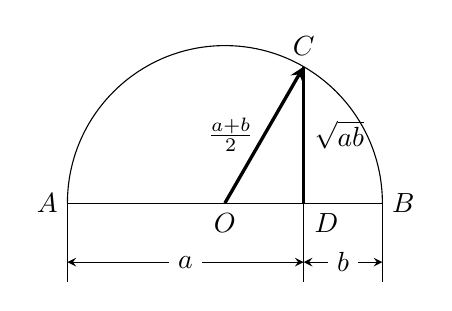
\begin{tikzpicture}[>=stealth]
\coordinate (A) at (-2,0);
\coordinate (O) at (0,0);
\coordinate (B) at (2,0);
\coordinate (D) at (1,0);
\coordinate (C) at (60:2);
\draw(B) arc (0:180:2);
\draw(A)node[left]{$A$}--(B)node[right]{$B$};
\draw[->, very thick](O)node[below]{$O$}--node[left]{$\frac{a+b}{2}$}(C)node[above]{$C$};
\draw(A)--+(0,-1);
\draw(D)--+(0,-1);
\draw(B)--+(0,-1);
\draw[<->](-2,-.75)--node[fill=white]{$a$}(1,-.75);
\draw[<->](1,-.75)--node[fill=white]{$b$}(2,-.75);
\draw[very thick](C)--node[right]{$\sqrt{ab}$}(D)node[below right]{$D$};


\end{tikzpicture}
    \caption{}
\end{figure}

\subsection{对平均不等式的认识}
先将上面的结果整理如下:
\begin{thm}{定理1}
    若$a$,$b$都是非负数,则
\begin{equation}
    \frac{a+b}{2}\ge \sqrt{ab}\qquad 
\text{(等号当且仅当$a=b$时成立)}\tag{1}
\end{equation}
进而还有:若$x,y\in\R$,则
\begin{equation}
    x^2+y^2\ge 2xy\qquad \text{(等号当且仅当$x=y$时成立)}\tag{2}
\end{equation}
\end{thm}

\begin{thm}{推论1 }
\[\begin{split}
    a\text{是正数}&\Longrightarrow a+\frac{1}{a}\ge 2\\
    a\text{是负数}&\Longrightarrow a+\frac{1}{a}\le -2
\end{split}\]
\end{thm}

\begin{thm}{推论2}
\[\begin{split}
    a,b\text{同号}&\Longrightarrow \frac{a}{b}+\frac{b}{a}\ge 2\\
a,b\text{异号} &\Longrightarrow \frac{a}{b}+\frac{b}{a}\ge -2\\
\end{split}\]
\end{thm}

\begin{thm}{定理2}
    若$a$,$b$,$c$都是非负数,则
\begin{equation}
    \frac{a+b+c}{3}\ge \sqrt[3]{abc}\tag{3}
\end{equation}
(等号当且仅当$a=b=c$时成立)
\end{thm}

(3)等价于:
若$x$,$y$,$z$都是非负数,则
\begin{equation}
    x^3+y^3+z^3\ge 3xyz \tag{4}
\end{equation}
(等号当且仅当$x=y=z$时成立)

更一般地有

\begin{thm}{定理3}
    若$a_1,a_2,\ldots,a_n$都是非负数,则
    \begin{equation}
\frac{a_1+a_2+\cdots +a_n}{n}\ge \sqrt[n]{a_1a_2\cdots a_n},\quad (n\in\N)       \tag{*}
    \end{equation}
当且仅当$a_1=a_2=\cdots= a_n$时等号成立。
\end{thm}
 
(*)等价于:若$x_1,x_2,\ldots,x_n$都是非负数,则
\begin{equation}
x^n_1+x^n_2+\cdots +x^n_n  \ge nx_1x_2\cdots x_n \tag{**}
\end{equation}
(等号当且仅当$x_1=x_2=\cdots=x_n$时成立)

对于(*)或(**),应特别注意理解:
\begin{enumerate}
    \item 式子的结构特征都是非负数的
\[\text{和的形式}\ge \text{积的形式}\]
若欲证不等式具有这样的结构特征,就有可能用“平均不等式”作出证明。这是能否利用“平均不等式”来证不等式的线索。
\item (*)或(**)还表明,$n$个非负数的和与积通过缩小或放大可以互相转化。认识了这一点用起(*)来就灵活多了。
\end{enumerate}


以下,举例说明怎样利用“平均不等式”去证明某些不等式.

\begin{example}
  求证下列不等式:  
\begin{enumerate}[(1)]
    \item $a^2+b^2+c^2\ge ab+bc+ca$
    \item 若$a$,$b$,$c$是不全相等的正数,求证
   \[ a(b^2+c^2)+b(c+a)+c(a^2+b^2)>6abc\]
    \item $a^4+b^4+c^4\ge abc(a+b+c)$,并指出等号成立的条件.
\end{enumerate}
\end{example}
 
\begin{proof}
\begin{enumerate}[(1)]
    \item 

    \begin{flushleft}
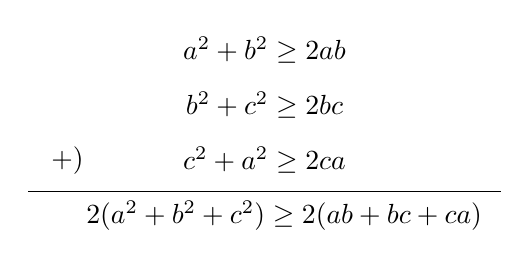
\begin{tikzpicture}
    \node at (-2.5, 3){$\because$};
\node at (0,3){$a^2+b^2\ge 2ab$};
\node at (0,2.3){$b^2+c^2\ge 2bc$};
\node at (0,1.6){$c^2+a^2\ge 2ca$};
\node at (.25,.9){$2(a^2+b^2+c^2)\ge 2(ab+bc+ca)$};
\draw(-3,1.2)--(3,1.2);
\node at (-2.5,1.6){$+)$};
\end{tikzpicture}
\end{flushleft}

$\therefore\quad a^2+b^2+c^2\ge ab+bc+ca$

\item \textbf{证法1:}由$b^2+c^2\ge 2bc,\; a>0$,得:
\[a(b^2+c^2)\ge 2abc\]
同理:
\[
    b(c^2+a^2)\ge 2abc, \qquad 
    c(a^2+b^2)\ge 2abc
\]

$\because\quad a,b,c$不全相等,

$\therefore\quad $上述三个不等式的等号不能同时成立。把三式左、右分别相加得
\[a(b^2+c^2)+b(c^2+a^2)+c(a^2+b^2)>6abc\]

\textbf{证法2:}$a,b,c$是不全相等的正数,


$\therefore\quad a(b^2+c^2),\; b(c^2+a^2),\; c(a^2+b^2)$也为正数。

由平均不等式($n=3$的情况)可得
\[    \begin{split}
a(b^2+c^2)+b(c^2+a^2)+c(a^2+b^2)&\ge 3\sqrt[3]{a(b^2+c^2)\cdot b(c^2+a^2)\cdot c(a^2+b^2)}\\
&>3\sqrt[3]{a(2bc)\cdot b(2ca)\cdot c(2ab)}\qquad \text{(理由?)}\\
&=3\sqrt[3]{(2abc)^3}=3\cdot 2abc=6abc
\end{split}\]
$\therefore\quad $原式成立.

\item $\because$
\begin{flushleft}
    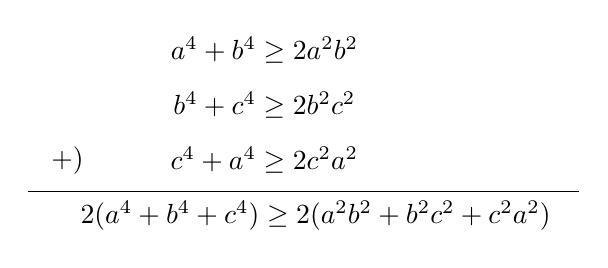
\begin{tikzpicture}
        % \node at (-2.5, 3){$\because$};
    \node at (0,3){$a^4+b^4\ge 2a^2b^2$};
    \node at (0,2.3){$b^4+c^4\ge 2b^2c^2$};
    \node at (0,1.6){$c^4+a^4\ge 2c^2a^2$};
    \node at (.65,.9){$2(a^4+b^4+c^4)\ge 2(a^2b^2+b^2c^2+c^2a^2)$};
    \draw(-3,1.2)--(4,1.2);
    \node at (-2.5,1.6){$+)$};
    \end{tikzpicture}
    \end{flushleft}
当且仅当$a^2=b^2=c^2$时等号成立.

而
\begin{flushleft}
    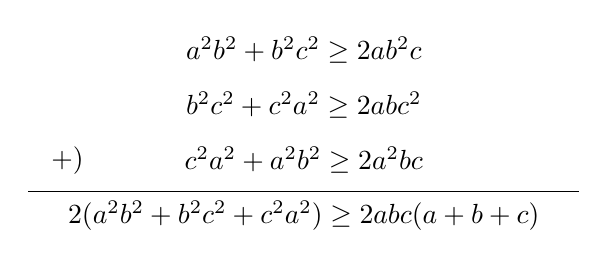
\begin{tikzpicture}
        % \node at (-2.5, 3){$\because$};
    \node at (0,3){$a^2b^2+b^2c^2\ge 2ab^2c$};
    \node at (0,2.3){$b^2c^2+c^2a^2\ge 2abc^2$};
    \node at (0,1.6){$c^2a^2+a^2b^2\ge 2a^2bc$};
    \node at (0,.9){$2(a^2b^2+b^2c^2+c^2a^2)\ge 2abc(a+b+c)$};
    \draw(-3.5,1.2)--(3.5,1.2);
    \node at (-3,1.6){$+)$};
    \end{tikzpicture}
    \end{flushleft}
当且仅当$ab=bc=ca$时等号成立。
由此,
$2(a^4+b^4+c^4)\ge 2abc(a+b+c)$,

$\therefore\quad a^4+b^4+c^4>abc(a+b+c)$,
当且仅当$a=b=c$时成立。
\end{enumerate}

\end{proof}

\begin{rmk}
    这三个小题式子的结构特征都是“和的形式$\ge $积的形式”的迭加,从而先用平均不等式,再迭加即可。
\end{rmk}

\begin{example}
    已知$a$,$b$,$c$为正数,求证:
\begin{enumerate}[(1)]
    \item $(a+b)(b+c)(c+a)\ge 8abc$;
    \item $(a+b+c)^4\cdot (a^2+b^2+c^2)\ge 243a^2b^2c^2$.
\end{enumerate}
\end{example}

\begin{analyze}
    这类不等式可看作是“和的形式$\ge $积的形式”经迭乘而成。
\end{analyze}

\begin{proof}
\begin{enumerate}[(1)]
    \item $\because\quad a>0,\; b>0,\; c>0$

$\therefore\quad a+b\ge 2\sqrt{ab}>0,\quad b+c\ge 2\sqrt{bc}>0,\quad c+a\ge 2\sqrt{ca}>0$

以上三式左、右分别相乘得
\[(a+b)(b+c)(c+a)\ge 8\sqrt{ab\cdot bc\cdot ca}=8abc\]
\item $\because\quad a,b,c$都是正数,

$\therefore\quad a+b+c\ge 3\sqrt[3]{abc}>0\Longrightarrow (a+b+c)^4\ge 3^4\cdot (abc)^{\tfrac{4}{3}}>0$

又$a^2+b^2+c^2\ge 3\sqrt[3]{a^2b^2c^2}=3(abc)^{\tfrac{2}{3}}>0$

以上三式左、右分别相乘得
\[(a+b+c)^4\cdot (a^2+b^2+c^2)\ge 3^4\cdot 3(abc)^{\tfrac{4}{3}\times \tfrac{3}{2}}=243a^2b^2c^2\]
\end{enumerate}
\end{proof}

\begin{example}
    求证:$\lg 9\cdot \lg 11<1$\hfill(1)
\end{example}

\begin{analyze}
因$\lg11>1$, $\lg9<1$,故用两式相乘得不出欲证结果,怎么办?这个题能否用“平均”去作?事实上,从(1)式的结构上看,左边是两个正数$\lg9$与$\lg11$的“积”,这与平均不等式的结构特征相似,因此可用“平均”去做。此时有两个不等式可供选用:
\[ab\le \frac{a^2+b^2}{2}\quad \text{或}\quad \sqrt{ab}\le\frac{a+b}{2}\]
\end{analyze}

\begin{proof}
\textbf{证法1:}
\begin{flushleft}
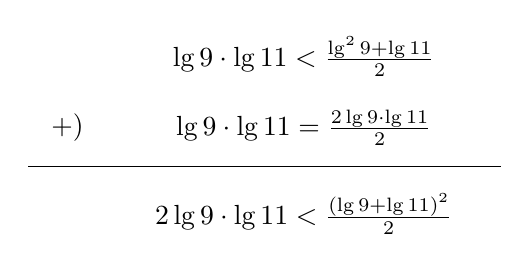
\begin{tikzpicture}
    \node at (0,2.2){$\lg 9\cdot \lg 11<\frac{\lg^2 9+\lg 11}{2}$};
    \node at (0,1.3){$\lg 9\cdot \lg 11=\frac{2\lg 9\cdot \lg 11}{2}$};
\node at (-3,1.3){$+)$};
\draw(-3.5,0.8)--(2.5,.8);
\node at (0,.2){$2\lg9\cdot \lg 11<\frac{(\lg 9+\lg 11)^2}{2}$};
\end{tikzpicture}
\end{flushleft}

于是:\[
    \frac{(\lg 9+\lg 11)^2}{2}=\frac{(\lg99)^2}{2}< \frac{\lg 100}{2}=\frac{2}{2}=1
\]
$\therefore\quad \lg 9\cdot \lg 11<1$

\textbf{证法2:}$\because\quad \lg 9>0,\; \lg 11>0$

$\therefore\quad \sqrt{\lg 9\cdot \lg 11}<\frac{\lg 9+\lg11}{2}=\frac{\lg 99}{2}<\frac{\lg 100}{2}=\frac{2}{2}=1$

两边平方得:$\lg 9\cdot \lg 11<1$
\end{proof}

\begin{blk}
你能把例4.12加以推广吗?
\end{blk}

\begin{example}
若$a>b>0$,求证$a+\frac{1}{(a-b)b}\ge 3$,并指出等号成立的条件.
\end{example}

\begin{analyze}
    $a+\frac{1}{(a-b)b}$可写成$(a-b)+b+\frac{1}{(a-b)b}$,且由于$a>b
    >0$,可知$a-b>0,\; b>0,\; \frac{1}{(a-b)b}>0$,所以,可用“平均”来做.
\end{analyze}

\begin{proof}
\[a+\frac{1}{(a-b)b}=(a-b)+b+\frac{1}{(a-b)b}\]

$\because\quad a>b>0$

$\therefore\quad a-b>0,\; b>0,\; \frac{1}{(a-b)b}>0$,可得
\[(a-b)+b+\frac{1}{(a-b)b}\ge 3\sqrt[3]{(a-b)\cdot b\cdot \frac{1}{(a-b)b}}=3\]
从而原式成立. 

当且仅当$a-b=b=\frac{1}{(a-b)b}$,即$a=2,\; b=1$时等号成立.
\end{proof}

\begin{rmk}
这个题的结构特征是在“$\ge $”号的左边是一个各项皆正的“和的形式”,而右边是个特征系数3。这就启示我们有可能用“平均”去做。方法是“凑”,使左边凑出一个三项和。
\end{rmk}

\section*{习题四}
\begin{center}
    \bfseries A
\end{center}

\begin{enumerate}
    \item 已知$a$,$b$,$c$,$d$都是正数,求证
    \[a^2+b^2+c^2+d^2\ge ab+bc+cd+da\]
    \item 已知$a,b,c\in\R$,求证
    $a^2+b^2+c^2+3\ge 2(a+b+c)$,并指出等号成立的条件。
    \item $a$,$b$都是正数,求证
    $a+b^2(a+1)+a^2(b+1)+b\ge 6ab$
    \item 若$a>1$, $b>1$, $c>1$,
    求证$(a+1)(b+1)(a+c)(b+c)>16abc$.
    \item 已知$a_1,a_2,\ldots, a_n$都是正数,求证:
    \[(a_1+a_2+\cdots +a_n)\left(\frac{1}{a_1}+\frac{1}{a_2}+\cdots+\frac{1}{a_n}\right)\ge n^2\]
    \item 已知$a$,$b$,$c$,$d$都是正数,求证:
    \begin{enumerate}[(1)]
        \item $(ab+cd)(ac+bd)\ge 4abcd$
        \item $\left(\frac{a}{c}+\frac{b}{c}+\frac{c}{d}+\frac{d}{a}\right)(a^3+b^3+c^3)\ge 12abc$
    \end{enumerate}  
\end{enumerate}

\begin{center}
    \bfseries B
\end{center}

\begin{enumerate}\setcounter{enumi}{6}
    \item 已知$a>0$,求证:
\begin{enumerate}[(1)]
    \item $a+\frac{4}{a^2}\ge 3$
    \item $a^4+\frac{4}{a^2}\ge 3\sqrt[3]{4}$
\end{enumerate}
\item 求证$\frac{x^2+2}{\sqrt{x^2+1}}\ge 2$,其中$x\in\R$
\item 若$x\in\R$,求证:$1+2x^4\ge x^2+2x^3$
\item 若$x,y\in\R^+$,求证:$\frac{1}{x}+\frac{1}{y}\ge \frac{4}{x+y}$
\item 当$a\ge 2$时,求证$\log_a(a-1)\cdot \log_a(a+1)<1$(这个题是例4.12的推广)
\item \begin{enumerate}[(1)]
    \item 若$a>b>c>d$,求证:$a-d+\frac{25^2}{(a-b)(b-c)(c-d)}\ge 20$
    \item 若$m>n>0$,求证:$m+n+\frac{16}{(m-n)n^2}\ge 8$
\end{enumerate}

\item 若$a,b,c$为三角形的三边,求证:
\begin{enumerate}[(1)]
    \item $(a+b+c)^3\ge 27(a+b-c)(b+c-a)(c+a-b)$
    \item $\frac{1}{a+b-c}+\frac{1}{b+c-a}+\frac{1}{c+a-b}\ge \frac{9}{a+b+c}$
\end{enumerate}

\end{enumerate}

\begin{center}
    \bfseries C
\end{center}

\begin{enumerate}\setcounter{enumi}{13}
    \item 若$x>0$,求证:$1+\frac{1+x}{9}>\sqrt[9]{2+x}$
    \item 对于任意正数$a,b$,$a\ne b$,求证$\sqrt[n+1]{ab^n}<\frac{a+nb}{n+1}$
    \item 若$a,b,c,d$为正数,求证:
\begin{enumerate}[(1)]
    \item $\frac{1}{a+b+c}+\frac{1}{b+c+d}+\frac{1}{c+d+a}+\frac{1}{d+a+b}\ge \frac{16}{3}\cdot \frac{1}{a+b+c+d}$
    \item $\frac{1}{a+3b+5c+7d}+\frac{1}{b+3c+5d+7a}+\frac{1}{c+3d+5a+7b}+\frac{1}{d+3a+5b+7c}\ge \frac{1}{a+b+c+d}$
\end{enumerate}
\end{enumerate}

\section{用放缩法证明不等式}

先研究一个例子。

\begin{example}
    若$a$,$b$,$c$,$d$为任意正数,求证
\[1<\frac{a}{a+b+c}+\frac{b}{b+c+d}+\frac{c}{c+d+a}+\frac{d}{d+a+b}<2\]
\end{example}

\begin{analyze}
    记$m=\frac{a}{a+b+c}+\frac{b}{b+c+d}+\frac{c}{c+d+a}+\frac{d}{d+a+b}$

这个题并不是让我们去求$m$的值,而是证明$m$的值存在的范围是在区间$(1,2)$之中,因而,就实质而言,这是一个“估值问题”。显然,先通分、求和再估值是不可取的。处理估值问题的方法,一般是对所给的式子的值先放大(或缩小),使之由繁化简,再进一步研究。
\end{analyze}

\begin{proof}
    由于$a$、$b$、$c$、$d$为正数,可先通过“放大”分母,把$m$缩小。
\[\begin{split}
    m&>\frac{a}{a+b+c+d}+\frac{b}{b+c+d+a}+\frac{c}{c+d+a+b}+\frac{d}{d+a+b+c}\\
    &=\frac{a+b+c+d}{a+b+c+d}=1
\end{split}\]
(“放大”之后构
造出公分母,实现了由繁化简)。再把分母“缩小”,达到把$m$放大.
\[m<\frac{a}{a+c}+\frac{b}{b+d}+\frac{c}{c+a}+\frac{d}{d+b}=\frac{a+c}{a+c}+\frac{b+d}{b+d}=2\]
$\therefore\quad 1<m<2$.
\end{proof}

\begin{thm}{放缩法原理}
由不等式的传递性,若$a>b$, $b>c$,则$a>c$. 由此,欲证$a>c$,可以先把$a$逐步缩小:
\[a>b_1>b_2>\cdots >b_n\]
而最后只要证出$b_n>c$,就可断言$a>c$. 类似地,欲证$a<c$,可以先把$a$逐步放大:
\[a<d_1<d_2<\cdots <d_n\]
最后,只要证出$d_n<c$,就可断言$a<c$.
\end{thm}

\begin{example}
    若$a\ge b>0$, $n\in\N$,求证
\begin{equation}
    n(a-b)b^{n-1}\le a^n-b^n\le n(a-b)a^{n-1}\tag{1}
\end{equation} 
\end{example}

\begin{proof}
    $\because\quad a\ge b>0$, $n\in\N$,且
\begin{equation}
    a^n-b^n=(a-b)(a^{n-1}+a^{n-2}b+a^{n-3}b^2+\cdots+ab^{n-2}+b^{n-1})  \tag{2}
\end{equation}
\begin{enumerate}[(i)]
\item 当$a=b$时,(1)式显然成立;
\item 当$a>b>0$时,(1)式等价于
\begin{equation}
nb^{n-1}\le a^{n-1}+a^{n-2}b+a^{n-3}b^2+\cdots+ab^{n-2}+b^{n-1}\le na^{n-1}\tag{3}
\end{equation}
\end{enumerate}
对(3)中间的和式使用放缩法,有
\[\begin{split}
    a^{n-1}+a^{n-2}b+a^{n-3}b^2+\cdots+ab^{n-2}+b^{n-1}&<a^{n-1}+a^{n-1}+\cdots+a^{n-1}=na^{n-1}\\
    a^{n-1}+a^{n-2}b+a^{n-3}b^2+\cdots+ab^{n-2}+b^{n-1}&>b^{n-1}+b^{n-1}+\cdots+b^{n-1}=nb^{n-1}\\
\end{split}\]

$\therefore\quad $(3)式成立,从而(1)式成立.
\end{proof}

\begin{example}
若$S_n=1+\frac{1}{\sqrt{2}}+\frac{1}{\sqrt{3}}+\cdots+\frac{1}{\sqrt{n}}$, $n\in\N$,求证:
\[2\left(\sqrt{n+1}-1\right)<S_n<2\sqrt{n}\]
\end{example}

\begin{analyze}
可把$S_n$看作是下面一列数
\[1,\; \frac{1}{\sqrt{2}},\; \frac{1}{\sqrt{3}}\cdots,  \frac{1}{\sqrt{n}}, \cdots\]
的前边$n$个项的和。这里并不要求计算$S_n$的精确值,而是估计$S_n$的值存在的范围。因而可用放缩法。由于$S_n$有$n$项,放缩后裂项相抵消是最理想的。
\end{analyze}

\begin{proof}
    先考虑上面一列数中的第$n$个项的通项怎样放缩(放缩的办法很多,下面的方法兼有裂项的目的)
\[\begin{split}
\frac{1}{\sqrt{k}} &= \frac{2}{\sqrt{k}+\sqrt{k}}<\frac{2}{\sqrt{k}+\sqrt{k-1}} =2(\sqrt{k}-\sqrt{k-1}) \\   
\frac{1}{\sqrt{k}} &=  \frac{2}{\sqrt{k}+\sqrt{k}}>\frac{2}{\sqrt{k}+\sqrt{k+1}} =2(\sqrt{k+1}-\sqrt{k}) \\    
\end{split}\]
再令$k=1,2,3,\ldots,n-1,n$,得:
\begin{flushleft}
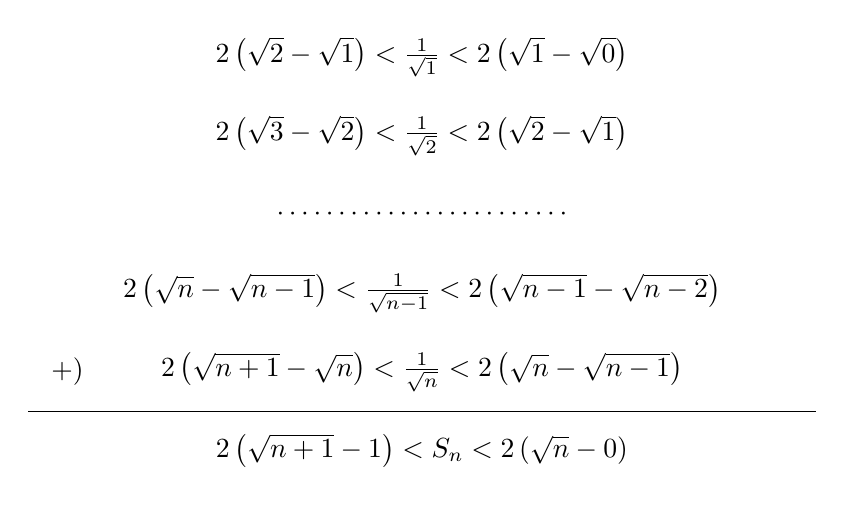
\begin{tikzpicture}
\node at (0,3){$2\left(\sqrt{2}-\sqrt{1}\right)<\frac{1}{\sqrt{1}}<2\left(\sqrt{1}-\sqrt{0}\right)$}  ;  
\node at (0,2){$2\left(\sqrt{3}-\sqrt{2}\right)<\frac{1}{\sqrt{2}}<2\left(\sqrt{2}-\sqrt{1}\right)$}  ;  
\node at (0,1){$\cdots \cdots\cdots \cdots\cdots \cdots\cdots \cdots$}  ;  
\node at (0,0){$2\left(\sqrt{n}-\sqrt{n-1}\right)<\frac{1}{\sqrt{n-1}}<2\left(\sqrt{n-1}-\sqrt{n-2}\right)$}  ;  
\node at (0,-1){$2\left(\sqrt{n+1}-\sqrt{n}\right)<\frac{1}{\sqrt{n}}<2\left(\sqrt{n}-\sqrt{n-1}\right)$}  ;  
\node at (-4.5,-1){$+)$}  ;  
\draw(-5,-1.5)--(5,-1.5);
\node at (0,-2){$2\left(\sqrt{n+1}-1\right)<S_n<2\left(\sqrt{n}-0\right)$};
\end{tikzpicture}
\end{flushleft}

$\therefore\quad 2\left(\sqrt{n+1}-1\right)<S_n<2\sqrt{n}$.

\end{proof}

\begin{rmk}
  这里的“放”或“缩”,由于把握了分式和根式的性质,使得求和成为可能。 
\end{rmk}

\section*{习题五}
\begin{center}
    \bfseries A
\end{center}

\begin{enumerate}
    \item 若$a>0$, $b>0$,求证:
\[\frac{a+b}{1+a+b}<\frac{a}{1+a}+\frac{b}{1+b}<\frac{2(a+b)}{1+a+b}\]
\item 求证:$-\sqrt{2}\le \sin x+\cos x\le \sqrt{2}$
\end{enumerate}

\begin{center}
    \bfseries B
\end{center}


\begin{enumerate}\setcounter{enumi}{2}
    \item 求证: $1\le \frac{1}{1^2}+ \frac{1}{2^2}+\cdots + \frac{1}{n^2}<2$
    
(提示:利用$k^2>k(k-1)$)

\item 求证:$1+\frac{1}{1!}+\frac{1}{2!}+\frac{1}{3!}+\cdots+\frac{1}{n!}<3$

(提示:利用$\frac{1}{n!}<\frac{1}{(n-1)n}$或$\frac{1}{n!}<\frac{1}{2^{n-1}}$)

\item 设$a_n=\sqrt{1\cdot 2}+\sqrt{2\cdot 3}+\cdots +\sqrt{n(n+1)}$,求证:
\[\frac{n(n+1)}{2}<a_n<\frac{(n+1)^2}{2}\quad (n\in\N)\]
\end{enumerate}

\begin{center}
    \bfseries C
\end{center}


\begin{enumerate}\setcounter{enumi}{5}
\item 若$x_n=\frac{n^2-n+2}{3n^2+2n-4}$,求证:当$n>2$时,有
\[\left|x_n-\frac{1}{3}\right|<\frac{1}{n}\]
(提示:对$|x_n-\tfrac{1}{3}|$连续放大)

\item 若$a,b,c\in\R^+$,求证:$\frac{a}{b+c}+\frac{b}{c+a}+\frac{c}{a+b}\ge \frac{3}{2}$.
\end{enumerate}

\section{* 柯西不等式}

作为选学内容,本节介绍著名的\textbf{柯西(Cauchy)不等式}。
若$a,b,x,y\in \R$, 则
\begin{equation}
    (ax+by)^2\le (a^2+b^2)(x^2+y^2)  \tag{1}
\end{equation}
(注意,这个不等式在本章习题三第13题曾证过)

现在,探索$(1)的新证法$。

(1)式的结构特征使我们联想到一元二次 方程 的 判别式
$\Delta=b^2-4ac$。由此,欲证(1), 只要证关于$t$的二次三项式
$$f(t)=(a^2+b^2)t^2-2(ax+by)t+(x^2+y^2)\ge 0$$
这一点可以通过对$f(t)$配方实现,
\[\begin{split}
    f(t)&=(a^{2}t^{2}-2axt+x^{2})+(b^{2}t^{2}-2byt+y^{2})\\
    &=(at-x)^{2}+(bt-y)^{2}\ge 0
\end{split}\]
等号当且仅当$at=x$, $bt=y$, 也就是$a$, $b$与$x$, $y$对应成比例
时成立。

\begin{rmk}
    由(1)式的结构特征联想到$\Delta$, 从而想到去构造二次三项式$f(t)$.
\end{rmk}

把(1)推广:当$a,b,c,x,y,z\in \R$时就有
\begin{equation}
    (ax+by+cz)^{2}\le (a^{2}+b^{2}+c^{2})(x^{2}+y^{2}+z^{2})\tag{2}
\end{equation}
(等号当且仅当$a,b,c$与$x,y,z$对应成比例时成立)

当$a_1,a_2,\ldots,a_n$与$x_1,x_2,\ldots,x_n\in \R$, 又有
\begin{equation}
    (a_1x_1+a_2x_2+\cdots+a_nx_n)^2\le (a_1^2+a_2^2+\cdots+a_n^2)(x_1^2+
x_{2}^{2}+\cdots+x_{m}^{2}) \tag{3}
\end{equation}
(等号当且仅当$a_1,a_2,\cdots,a_n$与$x_1,x_2,\cdots,x_n$对应成
比例时成立).

\begin{example}
    用柯西不等式证明:
\begin{enumerate}[(1)]
    \item 若$a,b,c,d\in \R^+$, 则$\sqrt(a+c)(b+d)\geqslant\sqrt{ab}+\sqrt{cd}$,
\item 若$a,b,c\in \R^{+}$, 则$(a+b+c)\left(\frac1a+\frac1b+\frac1c\right)\ge 9$
\end{enumerate}
\end{example}

\begin{analyze}
    能否使用柯西不等式,关键要认清柯西不等式的
结构特征。其中,由$(\quad)^{2}$到$(\quad)\cdot(\quad)$可视为“放大”,
反向用可视为“缩小”。
\end{analyze}


\begin{proof}
\begin{enumerate}[(1)]
    \item $\because\quad a, b, c, d\in \R^{+ }$, 欲证原 不 等 式 , 只 要 证 
$\left(\sqrt{ab}+\sqrt{cd}\right)^2\leq (a+c)(b+d)$

即证$\left(\sqrt{a}\cdot\sqrt{b}+\sqrt{c}\cdot\sqrt{d}\right)^{2}\le \left[\left(\sqrt{a}\right)^{2}+\left(\sqrt{c}\right)^{2}\right]\cdot \left[\left(\sqrt{b}\right)^{2}+\left(\sqrt{d}\right)^{2}\right]$

由柯西不等式知此式成立

$\therefore\quad $原不等式成立。
\item $\because\quad  a,b,c\in \R^{+}$,
\[\begin{split}
&\quad (a+b+c)\left(\frac{1}{a}+\frac{1}{b}+\frac{1}{c}\right)\\
&=\left[(\sqrt{a})^2+(\sqrt{b})^2+(\sqrt{c})^2\right]\left[\left(\frac{1}{\sqrt{a}}\right)^2+\left(\frac{1}{\sqrt{b}}\right)^2+\left(\frac{1}{\sqrt{c}}\right)^2\right]\\
&\ge \left[\sqrt{a}\cdot\frac{1}{\sqrt{a}}+\sqrt{b}\cdot\frac{1}{\sqrt{b}}+\sqrt{c}\cdot\frac{1}{\sqrt{c}}\right]^2 \qquad  \text{(柯西不等式)}\\
&=(1+1+1)^2=9
\end{split}\]
\end{enumerate}
\end{proof}

\section*{*习题六}
\begin{enumerate}
    \item 证明柯西不等式(2)
    \item 若$a\in \R$, 用两种方法证明$(1+a+a^2)^2\le 3(1+a^2+a^4)$
    \item 已知$a,b,c$是互不相等的正数, $s=a+b+c$, 求证
    $$\frac{s}{s-a}+\frac{s}{s-b}+\frac{s}{s-c}>\frac{9}{2}$$
    \item 若$c\ge 0,\; a\ge c,\; b\ge c$, 求证
    \[\sqrt{c(a-c)}+\sqrt{c(b-c)}\le \sqrt{ab}\]
    \item $a_{1},a_{2},\ldots,a_{n}, b_{1},b_{2},\ldots,b_{n}\in \R^{+}$, 求证
    \[\sqrt{a_{1}b_{1}}+\sqrt{a_{2}b_{2}}+\cdots+\sqrt{a_{n}b_{n}}\le \sqrt{a_{1}+a_{2}+\cdots+a_{n}}\cdot \sqrt{b_{1}+b_{2}+\cdots+b_{n}}\]
    \item $3a^{2}+2b^{2}+c^{2}=1$, 求$3a+2b+c$的最大值.
    \item 若$a,b,c\in \R^{+},\; n\in \N$, 且$f(n)=\lg \frac{a^n+b^n+c^n}{3}$,求证:$2f(n)\le f(2n)$
\end{enumerate}

\section{附加条件的不等式的证明}
这类问题除具有前述不等式论证的共性以外,怎样使用附加条件就成了解题的关键。利用条件的方法是多种多样的,但是把条件直接代入(或变形后代入)或从条件出发作有目标的变形(变“已知”为“所求”)是最常用的两种方法。

\begin{thm}
{问} 从条件$a,b\in\R^+$,且$a+b=1$出发,你能获得哪些结论?试试看。    
\end{thm}

\begin{example}
已知$a,b,c\in\R^+$,且$a+b+c=1$,求证
\begin{equation}
    \frac{1}{a}+\frac{1}{b}+\frac{1}{c}\ge 9
\end{equation}
\end{example}

\begin{analyze}
    应从已知和所求的结构特征悟出下面的几种证法来。
\end{analyze}

\begin{proof}
\textbf{证法1:}$\because\quad a+b+c=1$,以$(a+b+c)$代换(1)之左边的分子,得
\[\begin{split}
    \frac{1}{a}&=\frac{a+b+c}{a}=1+\frac{b}{a}+\frac{c}{a}\\
    \frac{1}{b}&=\frac{a+b+c}{b}=1+\frac{a}{b}+\frac{c}{b}\\
    \frac{1}{c}&=\frac{a+b+c}{c}=1+\frac{a}{c}+\frac{b}{c}
\end{split} \]
以上三式,左、右分别相加,得
\begin{equation}
    \frac{1}{a}+\frac{1}{b}+\frac{1}{c}=3+\left(\frac{b}{a}+\frac{c}{a}\right)+\left(\frac{a}{b}+\frac{c}{b}\right)+\left(\frac{a}{c}+\frac{b}{c}\right) \tag{2}
\end{equation}

又$\because\quad a,b,c$都是正数,

$\therefore\quad \frac{b}{a}+\frac{c}{a}\ge 2,\quad \frac{a}{b}+\frac{c}{b}\ge 2,\quad \frac{a}{c}+\frac{b}{c}\ge 2$

代入(2)式得:$ \frac{1}{a}+\frac{1}{b}+\frac{1}{c}\ge 3+2+2+2=9$.

\textbf{证法2:} 已知$a+b+c=1$,代入(1)之左边
\[\begin{split}
    \frac{1}{a}+\frac{1}{b}+\frac{1}{c}&=\frac{a+b+c}{a}+\frac{a+b+c}{b}+\frac{a+b+c}{c}\\
    &=(a+b+c)\left(\frac{1}{a}+\frac{1}{b}+\frac{1}{c}\right)
\end{split}\]
又$a,b,c$都是正数,因而
\[a+b+c\ge 3\sqrt[3]{abc},\quad \frac{1}{a}+\frac{1}{b}+\frac{1}{c}\ge \sqrt[3]{\frac{1}{abc}}\]
从而:$$\frac{1}{a}+\frac{1}{b}+\frac{1}{c}\ge 3\sqrt[3]{abc}\cdot 3\sqrt[3]{\frac{1}{abc}}=9\sqrt[3]{abc\cdot \frac{1}{abc}}=9$$

\textbf{证法3:}$\because\quad a,b,c$都是正数,

$\therefore\quad \frac{1}{a}+\frac{1}{b}+\frac{1}{c}\ge 3\sqrt[3]{\frac{1}{abc}}=3\cdot \frac{1}{\sqrt[3]{abc}}$ \hfill (3)

又$\because\quad a+b+c=1$,利用$a+b+c\ge 3\sqrt[3]{abc}$可得
\begin{equation}
    1\ge 3\sqrt[3]{abc} \Longrightarrow \frac{1}{\sqrt[3]{abc}}\ge 3 \tag{4}
\end{equation}
由(3)(4)得:$\frac{1}{a}+\frac{1}{b}+\frac{1}{c}\ge 3\cdot \frac{1}{\sqrt[3]{abc}}\ge 3\cdot 3=9$
\end{proof}

\begin{example}
    $a,b,c,d,x,y$都是正数,且$x^2=a^2+b^2$, $y^2=c^2+d^2$,求证:
\begin{equation}
    xy\ge ac+bd \tag{1}
\end{equation}
\end{example}

\begin{analyze}
由条件的结构特征容易使我们联想到直角三角形,从而可以实行“三角换元”。
\end{analyze}

\begin{proof}
    由于$x^2=a^2+b^2,\quad y^2=c^2+d^2$,且$a,b,c,d,x,y$皆正,

设$\begin{cases}
    a=x\cos\alpha\\
    b=x\sin\alpha
\end{cases},\quad \begin{cases}
    c=y\cos\beta\\
    d=y\sin\beta
\end{cases}$(图4.3,$\alpha,\beta$为锐角)

\begin{figure}[htp]
    \centering
\begin{tikzpicture}[scale=.7]
\begin{scope}
\tkzDefPoints{0/0/A, 3/0/B, 3/2/C}
    \draw[very thick](A)--node[below]{$a$}(B)--node[right]{$b$}(C)--node[above]{$x$}cycle;
    \tkzMarkAngle[mark={}](B,A,C)
    \tkzLabelAngle[pos=1.5](B,A,C){$\alpha$}
    \tkzMarkRightAngle(C,B,A)
\end{scope}
\begin{scope}[xshift=5cm]
\tkzDefPoints{0/0/A, 5/0/B, 5/4/C}
    \draw[very thick](A)--node[below]{$c$}(B)--node[right]{$d$}(C)--node[above]{$y$}cycle;
    \tkzMarkAngles[mark={}](B,A,C)
    \tkzMarkRightAngle(C,B,A)
    \tkzLabelAngles[pos=1.5](B,A,C){$\beta$}
\end{scope}
\end{tikzpicture}
    \caption{}
\end{figure}

代入(1),
\[\begin{split}
    \text{右边}= ac+bd&=xy\cos\alpha\cos\beta+xy\sin\alpha\sin\beta\\
    &=xy\cos(\alpha-\beta)\le xy
\end{split}\]
$\therefore\quad $(1)成立.
\end{proof}

\begin{rmk}
    实行三角换元是高中数学中很重要的思想方法。
\end{rmk}

\begin{blk}
    若从结论入手,运用分析法,你能想出例4.19的新证法吗?
\end{blk}

\begin{example}
已知$x,y\in\R$且$x+y+z=2$,$x^2+y^2+z^2=2$,求证:$x,y,z$都不能是负数,也都不能大于$\frac{4}{3}$.
\end{example}

\begin{analyze}
    “元”多,是个难点,但$x$、$y$、$z$地位 对等,只要证出一个元满足关系即可——这就使我们想到消元。消元后出现二元二次方程,从而可用判别式法。
\end{analyze}

\begin{proof}
    由已知条件消去$x$得
$$y^{2}+\left(z-2\right)y+z^{2}-2z+1=0$$
这是关于y的一元二次方程.

$\because\quad y\in \R$,

$\therefore\quad \Delta = ( z- 2) ^{2}- 4\cdot 1\cdot ( z^{2}- 2z+ 1) \geq 0$

即   $-3z^2+4z\geq0$

$\therefore\quad 0\leq z\leq\frac{4}{3}$.

由已知可见$x,y,z$地位对等。同理可得:
$$0\le  y\le \frac{4}{3},\qquad 0\le  z\le \frac{4}{3}.$$
\end{proof}


\begin{example}
    若$x,y,z\in \R$, $A+B+C=\pi$, 求证
\begin{equation}
    x^2+ y^2+ z^2\geqslant 2yz\cos A+ 2zx\cos B+ 2xy\cos C.\tag{1}
\end{equation}
\end{example}

\begin{analyze}
    “元”多是(1)式的特点。若把$x$视为“主元”, 这就
是一元二次不等式.
\end{analyze}

\begin{proof}
欲证(1), 只要证明
\begin{equation}
    x^2-2(z\cos B+y\cos C)x+y^2+z^2-2yz\cos A \geq 0 \tag{2}
\end{equation}
这是关于$x$的二次不等式,

$\because \quad x^2$的系数$>0$,  
  
$\therefore\quad $欲证(2),只要证明$\Delta\le 0$,而
\[\begin{split}
    \Delta &= 4(z\cos B+y\cos C)^2-4\cdot1\cdot(y^2+z^2-2yz\cos A)\\
&= 4[ - z^{2}\sin ^{2}B- y^{2}\sin ^{2}C+ 2y\boldsymbol{z}( \cos A+ \cos B\cos C) ]
\end{split}\]

$\because\quad A+ B+ C= \pi $,

$\therefore\quad \cos A= \cos [ \pi - ( B+ C) ] = - \cos ( B+ C)=-\cos B\cos C+\sin B\sin C$,

代入上式,
\[\begin{split}
    \Delta&=-4[z^{2}\sin^{2}B+y^{2}\sin^{2}C-2yz\sin B\sin C]\\
    &=-4(z\sin B-y\sin C)^{2}\le 0
\end{split}\]
从而(1)式成立.
\end{proof}

\begin{blk}
    对(2)式运用“配方法”能完成证明吗?试试看.
\end{blk}

\begin{example}
若$a,b,c\in\R$,且
\begin{equation}
    a\left(\frac{1}{b}+\frac{1}{c}\right)+
    b\left(\frac{1}{c}+\frac{1}{a}\right)+
    c\left(\frac{1}{a}+\frac{1}{b}\right)+3=0  \tag{1}
\end{equation}
求证:$ab+bc+ca\le 0$
\end{example}

\begin{analyze}
    为充分利用式子的对称性,可把条件中的“3”写成
\[a\cdot \frac{1}{a}+b\cdot \frac{1}{b}+c\cdot \frac{1}{c}\]
\end{analyze}

\begin{proof}
    把条件式写成
\[a\left(\frac{1}{a}+\frac{1}{b}+\frac{1}{c}\right)+b\left(\frac{1}{a}+\frac{1}{b}+\frac{1}{c}\right)+c\left(\frac{1}{a}+\frac{1}{b}+\frac{1}{c}\right)=0\]
即:$(a+b+c)\left(\frac{1}{a}+\frac{1}{b}+\frac{1}{c}\right)=0\Longrightarrow (a+b+c)\cdot \frac{ab+bc+ca}{abc}=0$

\begin{enumerate}
    \item 若$ab+bc+ca=0$,则命题(1)成立;
    \item 若$a+b+c=0$,则$(a+b+c)^2=0$,即$a^2+b^2+c^2+2(ab+bc+ca)=0$
    
    $\therefore\quad ab+bc+ca=-\frac{1}{2}(a^2+b^2+c^2)\le 0$
\end{enumerate}
综上所述,(1)成立。
\end{proof}

\section*{习题七}
\begin{center}
    \bfseries A
\end{center}

\begin{enumerate}
    \item 若$a,b,c\in\R^+$,且$a+b+c=1$,求证:$(1-a)(1-b)(1-c)\ge 8abc$
    \item 若$a,b,c\in\R^+$,且$abc=1$,求证:$(1+a)(1+b)(1+c)\ge 8$
    \item 若$a,b,c\in\R^+$,且$ab+bc+ca=1$,求证:$a+b+c\ge \sqrt{3}$
    \item 若$a,b,c\in\R^+$,且$a+b+c=1$,求证:
\begin{enumerate}[(1)]
    \item $\frac{1}{a^2}+\frac{1}{b^2}+\frac{1}{c^2}\ge 27$
    \item $a^2+b^2+c^2\ge \frac{1}{3}$
    \item $ab+bc+ca\le \frac{1}{3}$
    \item $\left(\frac{1}{a}-1\right)\left(\frac{1}{b}-1\right)\left(\frac{1}{c}-1\right)\ge 8$
\end{enumerate}    
    \item 若$a,b\in\R^+$,且$a+b=1$,求证:$\left(1+\frac{1}{a}\right)\left(1+\frac{1}{b}\right)\ge 9$
    \item 若$a>b>c$,求证:$\frac{1}{a-b}+\frac{1}{b-c}\ge \frac{4}{a-c}$
\end{enumerate}

\begin{center}
    \bfseries B
\end{center}

\begin{enumerate}
 \setcounter{enumi}{6}   
 \item \begin{enumerate}[(1)]
     \item 若$a,b$都是非负数,且$a+b=1$,求证:$1\le \sqrt{a}+\sqrt{b}\le \sqrt{2}$.
     \item 对(1),你还能推广吗?
 \end{enumerate}
 \item 若$a,b,c\in\R^+$,且$a+b+c=3$,求证:$\sqrt{3a-2}+\sqrt{3b-2}+\sqrt{3c-2}\le 3$
 \item 用三角换元法证明(结构上的什么特征使你能联想到三角换元?):
 \begin{enumerate}[(1)]
     \item 若$a^2+b^2=1$,$x^2+y^2=1$,$a,b,x,y\in\R$,则$|ax+by|\le 1$,此题还能推广吗?
     \item 若$x^2+y^2\le 1$,则$|x^2-2xy-y^2|\le \sqrt{2}$
     \item 若$|a|\le 1$, $|b|\le 1$,则$ab+\sqrt{(1-a^2)(1-b^2)}\le 1$
 \end{enumerate}

\item 已知$a,b$都是非负数,且$a+b=1$,求证:$(ax+by)(ay+bx)\ge xy$
\item 若$a>b>0$,且$ab=1$,求证:$\frac{a^2+b^2}{a-b}\ge 2\sqrt{2}$,并指出等号成立的条件.
\item 若$a,b,c\in\R$,$a+b+c=0$,$abc=1$,求证:$a,b,c$中必有一个大于3/2.
\item 设$a\ge b>0$,求$f(x)=(a-b)\sqrt{1-x^2}+ax$的最大值.
\end{enumerate}

\section{*平方平均数}
\begin{thm}{定义}
  $a_1,a_2,\ldots , a_n$是$n$个非负数,$\sqrt{\frac{a^2_1+a^2_2+\cdots+a^2_n}{n}}$叫做这$n$个数的\textbf{平方平均数}。
\end{thm}

\begin{example}
    若$a$,$b$是两个非负数,求证
    \begin{equation}
        \frac{a+b}{2}\le \sqrt{\frac{a^2+b^2}{2}}\tag{1}
    \end{equation}
\end{example}

\begin{proof}
\[\frac{a+b}{2}=\sqrt{\left(\frac{a+b}{2}\right)^2}=\sqrt{\frac{a^2+b^2+2ab}{4}}\le \sqrt{\frac{a^2+b^2+a^2+b^2}{4}}=\sqrt{\frac{a^2+b^2}{2}}\]
(等号当且仅当$a=b$时成立)
\end{proof}

设$0<a<b$,则$a,b$的几何平均、算术平均、平方平均与$a,b$的大小关系如图4.4所示(这有助于你记住它们之间的大小顺序)
\begin{figure}[htp]
    \centering
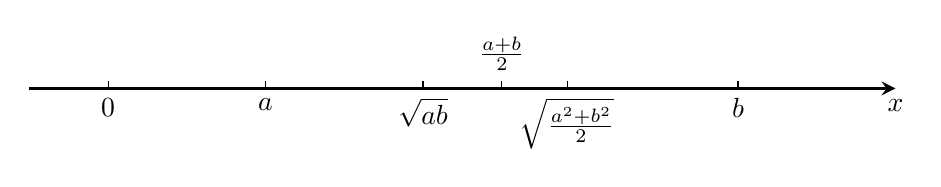
\begin{tikzpicture}[>=stealth]
    \draw[->, very thick](-1,0)--(10,0)node[below]{$x$};
    \foreach \x/\y in {0/0, 8/b, 2/a, 4/\sqrt{ab}, 5.83/\sqrt{\frac{a^2+b^2}{2}}}
    {
        \draw(\x,0)node[below]{$\y$}--(\x,.1);
    }
    \draw(5,0)--(5,.1)node[above]{$\frac{a+b}{2}$};
\end{tikzpicture}
    \caption{}
\end{figure}

从(1)式的结构特征可以看出$\frac{a+b}{2}$与$\frac{a^2+b^2}{2}$通过放大或缩小在形式上可以互化。这就为解题提供了方便。

若将(1)式中字母的次数推广,可得
\begin{equation}
    \frac{a+b}{2}\le \sqrt[3]{\frac{a^3+b^3}{2}} \tag{2}
\end{equation}

若将(1)式中字母的个数推广,可得
\begin{equation}
    \frac{a+b+c}{3}\le \sqrt{\frac{a^2+b^2+c^2}{3}}\tag{3}
\end{equation}

\begin{example}
若$a>0$, $b>0$, $a+b=1$,求证:
\begin{equation}
    \left(a+\frac{1}{a}\right)^2 +
    \left(b+\frac{1}{b}\right)^2 \ge \frac{25}{2}
\end{equation}
\end{example}

\begin{analyze}
直接展开左边,把条件代入,则运算较繁。(4)式的结构特征启发我们,有可能用“平方平均>算术平均”来证。为此,把(4)变形,先凑出平方平均数。
\end{analyze}

\begin{proof}
    欲证(4),等价于证明
\begin{equation}
    \sqrt{\frac{\left(a+\frac{1}{a}\right)^2 +    \left(b+\frac{1}{b}\right)^2}{2}}\ge \sqrt{\frac{25}{4}}=\frac{5}{2}
\end{equation}
对左边运用“平方平均$\ge $算术平均”,得
\[\sqrt{\frac{\left(a+\frac{1}{a}\right)^2 +    \left(b+\frac{1}{b}\right)^2}{2}}\ge \frac{\left(a+\frac{1}{a}\right) +    \left(b+\frac{1}{b}\right)}{2}=\frac{(a+b)+\left(\frac{1}{a}+\frac{1}{b}\right)}{2}\]

$\because\quad a>0,\; b>0,\; a+b=1$,利用上节的方法,可得:
\[\frac{\left(a+\frac{1}{a}\right) +    \left(b+\frac{1}{b}\right)}{2}\ge \frac{1+4}{2}=\frac{5}{2}\]

$\therefore\quad $(5)成立,从而(4)成立.
\end{proof}

\section*{习题八}
\begin{enumerate}
    \item 若$a+b+1=0$,求证:$\sqrt{(a-1)^2+(b-1)^2}\ge \frac{3}{\sqrt{2}}$.
    \item 若$a,b,c$为非负数,证明:$\frac{a+b+c}{3}\le \sqrt{\frac{a^2+b^2+c^2}{3}}$,再推广一步试试看.
    \item 若$a,b,c\in\R^+$,且$a+b+c=1$,试证:
    \[\left(a+\frac{1}{a}\right)^2+\left(b+\frac{1}{b}\right)^2+\left(c+\frac{1}{c}\right)^2\ge \frac{100}{3}\]
    \item 若$a,b,c\in\R^+$,且$a+b+c=1$,试证:$\frac{a+b}{2}\le \sqrt[3]{\frac{a^3+b^3}{2}}$ (右边称为“立方平均数”)
    
    这一结论再推广可能得到什么?
    \item 若$a\ge b\ge 0$,依照从小到大的顺序用“$\le $”号连接下列各式:
\[a,\; b,\; \frac{a+b}{2},\; \sqrt{ab},\; \sqrt{\frac{a^2+b^2}{2}}\]
\end{enumerate}


\section{同解不等式}

什么是同解方程?关于同解方程有几个基本定理?证明
这些定理的方法是什么?这个问题涉及到解方程的理论根据。

类似于方程,对于不等式我们有

\begin{thm}{定义} 
    如果两个不等式的解集相等,那么,这两个不等式叫做\textbf{同解不等式}。或者简称这两个不等式\textbf{同解},或者\textbf{等价}. 两个不等式$A$,$B$同解(或等价),可以用$A\Longleftrightarrow B$来表示。
\end{thm}

关于同解不等式,有下面几个基本定理。

\begin{thm}{定理1}
    不等式$f(x)>g(x)$与$g(x)<f(x)$同解。
\end{thm}

\begin{analyze}
    根据定义,要证这两个不等式同解,必须证明它们的解集相等。
\end{analyze}

\begin{proof}
\begin{enumerate}[(i)]
    \item 设$x=a$是$f(x)>g(x)$的任何一个解,则$f(a)>g(a)$,由不等式的性质知$g(a)<f(a)$,即$x=a$也是$g(x)<f(x)$解。

    \item 设$x=b$是$g(x)<f(x)$的任何一个解,即有$g(b)<f(b)$,则$f(b)>g(b)$,
    
    $\therefore\quad x=b$也是$f(x)>g(x)$的解.
\end{enumerate}
综合(i)、(ii),知道两个不等式的解集相等。

$\therefore\quad f(x)>g(x)\Longleftrightarrow g(x)<f(x)$
\end{proof}

\begin{thm}{定理2}
    不等式$f(x)>g(x)$与$f(x)+m>g(x)+m$(其中$m$是常数)同解。
\end{thm}

\begin{thm}{推论}
  把定理中的常数$m$换成函数$m(x)$后,若所得不等式与原不等式的未知数的取值范围相同(即不等式两边同加$m(x)$后,不等式的未知数的取值范围既不扩大,也不缩小),则两不等式同解。  
\end{thm}

\begin{note}
\begin{enumerate}[(1)]
\item 用定理1的证明方法可以证明这个定理及推论;
\item 要特别注意推论中对函数式$m(x)$所要求的条件。如不等式
\[2x+8>5x+2\quad \text{与}\quad 22x+8+\frac{4}{x-1}>5x+2+\frac{4}{x-1}\]
就不一定同解。事实上,前一个不等式的未知数的取值范围为实数集$\R$,而后一个的未知数的取值范围是$x\in\R$,且$x\ne 1$. 但是,
\[\frac{3}{x-1}>\frac{x+2}{x-2}\quad \text{与}\quad \frac{3}{x-1}+\frac{3x-4}{x-1}>\frac{x+2}{x-2}+\frac{3x-4}{x-1}\]
是同解的。这是因为前一个不等式两边同加$m(x)=\frac{3x-4}{x-1}$后,两个不等式的未知数的取值范围相同。
\item 定理2及其推论是“移项”的理论根据。
\end{enumerate}
\end{note}

\begin{thm}{定理3}
\begin{enumerate}
    \item 当常数$k>0$时,不等式$f(x)>g(x)$与$kf(x)>kg(x)$同解;
    \item 当常数$k<0$时,$f(x)>g(x)$与$kf(x)<kg(x)$同解.
\end{enumerate}
\end{thm}

\begin{thm}{推论}
    把定理中的常数$k$,分别换成在不等式的未知数的取值范围上解析式$k(x)$的值恒正或恒负时,定理的结论仍成立。    
\end{thm}

\begin{note}
\begin{enumerate}[(1)]
    \item 定理3和推论的证明方法同定理1;
    \item 运用定理3及其推论解不等式时,条件必须掌握好,如:

    解不等式$\frac1x>1$。不等式的未知数的取值范围是$x\neq0$, 用$k\left(x\right)=x$乘两边,这时$k\left(x\right)$在未知数的取值范围上不是恒正或恒负,因此必须对$k(x)$分两种情况进行讨论:
    \begin{enumerate}[(i)]
    \item 当$x>0$时,$\frac1x>1{\Longleftrightarrow}x\cdot\frac1x{>}x{\cdot}1{\Longleftrightarrow}1{>}x$,
    所以$0<x<1$,
    \item 当$x<0$时,$-\frac1x>1\Longleftrightarrow x\cdot\frac1x<x\cdot1\Longleftrightarrow1<x$, 所以无解。
    \end{enumerate}
    综合(i)、(ii), 知原不等式的解是$0<x<1$.
    
    由此可见,这样讨论是较繁的,特别当所用的$k(x)$较复杂时就更繁。因此解分式不等式,我们一般不采用以$k(x)$乘两边(去分母)的办法。
\end{enumerate}
\end{note}

\begin{thm}{定理4}
\begin{enumerate}[(i)]
    \item 不等式 $\frac {f(x)}{g(x)}>0$ 与$f(x)g(x)>0$同解
    \item 不等式$\frac {f(x)}{g(x)}<0$与$f(x)g(x)<0$同解。
\end{enumerate}
\end{thm}

\begin{note}
    定理 4 的证明方法同定理 1, 此定理是将分式不
等式转化为整式不等式的依据。
\end{note}

\begin{thm}{定理5 }
 当$f(x)$与$g(x)$ 在不等式 $f(x)>g(x)$ 的未知数的取值范围上都非负时,$f(x)>g(x)\Longleftrightarrow f^n(x)>g^n(x)$, $n\in \N$.   
\end{thm}

\begin{note}
\begin{enumerate}[(1)]
    \item 定理 5 的证明方法同定理1。
\item 若$f(x), g(x)$在未知数的取值范围上非正,对$f(x)>g(x)$两边同乘$(-1)$变成非负解决之.
\item 这个定理是将无理不等式转化为有理不等式的依据。但在运用定理时,必须掌握好定理的条件。
\end{enumerate} 
\end{note}


    对于这五个基本定理,再做几点说明:
\begin{enumerate}[(1)]
\item 定理1所起的作用如同不等式的性质中定理1一样,有了它,对“$>$”类型的不等式所成立的定理2,对“$<$”类型的不等式仍然成立。
\item 五个定理中,若把“$>$”改成“$\ge $”,定理1、2、3、5仍成立,但定理4不然。
\item 定理2、3、5中的条件,都涉及原不等式中未知数的取值范围。
\end{enumerate}

    以下几节,我们将学习各类代数不等式和指数、对数不等式的解法。作为基础,先研究两个例题。

\begin{example}
    解关于$x$的不等式
$ax>b$, 
其中$a$,$b$为任意实数。
\end{example}

\begin{solution}
\begin{enumerate}[(i)]
    \item 若$a>0$,则$x>\frac{b}{a}$\hfill(定理3)

    $\therefore\quad $解集为$\left(\frac{b}{a},+\infty\right)$
\item 若$a<0$,则$x<\frac{b}{a}$\hfill(定理3)

$\therefore\quad $解集为$\left(-\infty, \frac{b}{a}\right)$
\item 若$a=0,\; b<0$,任取$x\in\R$, $ax>b$式都成立,

$\therefore\quad $解集为$\R$.
\item 若$a=0,\; b\ge 0$,任取$ax>b$都不成立,

$\therefore\quad $解集为$\emptyset$.
\end{enumerate}
上述四种情况在解不等式时,是经常有用的。
\end{solution}

\begin{example}
    解关于$x$的不等式$mx-2>x-3m$ \hfill(1)
\end{example}

\begin{solution}
    $(1)\Longleftrightarrow (m-1)x>2-3m$\hfill (2)
\begin{enumerate}[(i)]
    \item 若$m-1>0$, $x>\frac{2-3m}{m-1}$
    \item 若$m-1<0$, $x<\frac{2-3m}{m-1}$
    \item 若$m-1=0$,即:$m=1$时,

$\because\quad     2-3m=2-3\x1=-1$,

$\therefore\quad  x$为任意实数。   
\end{enumerate}

从而:当$m>1$时,解集为$\left(\frac{2-3m}{m-1},+\infty\right)$;
当$m<1$时,解集为$\left(-\infty, \frac{2-3m}{m-1}\right)$;
当$m=1$时,解集为$\R$.
\end{solution}

\section*{习题九}
\begin{center}
    \bfseries A
\end{center}

\begin{enumerate}
\begin{multicols}{2}
    \item 解不等式组
\[\begin{cases}
    x>2\\ x<13\\ x>5\\ x<8
\end{cases}\]
    \item 解下列不等式组
\begin{enumerate}[(1)]
    \item $\begin{cases}
        2x+4>7x+3\\ 5x+6>6x+5\\ 8x-2<9x-4
    \end{cases}$
    \item $\begin{cases}
        x+2\ge \frac{x-9}{6}+\frac{x+4}{2}\\
        6-\left(\frac{x-2}{4}+\frac{2}{3}\right)\ge \frac{x}{6}
    \end{cases}$

    并求出它的整数解.
    \item $3x-1>2-\frac{x+1}{3}\ge 1-\frac{2x-3}{2}$
    \item $-12\le 3\frac{1}{3}x-5\le 4$
\end{enumerate}
    \item 解下列关于$x$的不等式    
    \begin{enumerate}[(1)]
        \item $ax+b^2>bx+a^2$
        \item $2k-3x>5-kx$
        \item $mx+4<m-2x$
        \item $m(mx-1)<2(2x-1)$
    \end{enumerate}
\end{multicols}
\end{enumerate}

